\documentclass[aps,prd,twocolumn,10pt,nofootinbib,superscriptaddress,floatfix]{revtex4-2}

\usepackage{amsmath,amssymb,bm}
\usepackage{graphicx}
\usepackage{booktabs}
\usepackage[colorlinks=true,linkcolor=blue,citecolor=blue,urlcolor=blue]{hyperref}

\newcommand{\dd}{\mathrm{d}}
\newcommand{\ii}{\mathrm{i}}
\newcommand{\calO}{\mathcal{O}}
\newcommand{\rp}{r_+}
\newcommand{\rmn}{r_-}
\newcommand{\OmH}{\Omega_H}
\newcommand{\Bin}{B^{\rm inc}}
\newcommand{\Bref}{B^{\rm ref}}
\newcommand{\Aref}{A_{\rm ref}^{(1)}}
\newcommand{\AH}{A_H^{(1)}}
\newcommand{\DeltaK}{\Delta}
\newcommand{\Res}{\mathcal R}

\begin{document}

\title{Nonlinear scalar scattering on Kerr: resonant response, frequency tails, and principal-mode enhancement}
\author{Jing-Qi Lai}
\email{laijingqi19@mails.ucas.ac.cn}
\affiliation{School of Physical Sciences, University of Chinese Academy of Sciences, Beijing 100049, China}
\author{Yu Tian}
\email[Corresponding author: ]{ytian@ucas.ac.cn}
\affiliation{School of Physical Sciences, University of Chinese Academy of Sciences, Beijing 100049, China}
\affiliation{Institute of Theoretical Physics, Chinese Academy of Sciences, Beijing 100190, China}

\begin{abstract}
We investigate the first-order scalar energy-flux response to local
interactions $|\Phi|^{2n}\Phi$ on a fixed Kerr background across the infrared,
resonance, and post-resonance frequency regimes.
For cubic axisymmetric scattering at $a/M=0.5$, $\ell=0,1,2$, the nonlinear
absorption has Breit--Wigner-type peaks near the fundamental scalar
quasinormal-mode frequency scale.  Post-resonance tails favor an
exponential over a power law in the tested windows.  An exact Green-function
decomposition separates flux and phase corrections.  Algebraic-prefactor tests
quantify the dependence of the fitted decay scale on the tail model.
At fixed incident amplitude and subextremal spin, cubic axisymmetric
absorption and its first-order correction have the same
$(M\omega)^{2\ell+2}$ power, with a spin-independent limiting ratio.
For the monopole this ratio is $\ln2/\pi$; higher interaction powers give
$M^{2n-2}\chi_{H,00}^{(n)}\sim c_n(M\omega)^{2n-2}$.
Near extremality at fixed $p/\kappa$, principal modes with
$h=1/2+i\beta$ concentrate the incident-normalized field in the throat.
Matching hypergeometric and Whittaker solutions and evaluating the
nonlinear Green integral give
$\widehat\chi_n=\sigma^{-n}{\cal F}_n(p/\kappa,\beta\ln\sigma)
+o(\sigma^{-n})$, where $\sigma=(r_+-r_-)/M$.
The coefficient has logarithmic period $\pi/\beta$ and is specified with
zero fitted parameters.  Spectral calculations test $(\ell,m)=(2,2),(3,3),(4,4)$,
$n=1,2,3$, and both signs of the horizon detuning.  Independent spectral
and quadrature refinements, coefficient tails, field-dependent radial
residuals and flux interference checks quantify numerical accuracy.
The enhancement identifies a shrinking weak-coupling domain near extremality.
Flux-response zeros coexist with enhanced phase coefficients at selected
near-critical detunings.
All results use fixed asymptotic incident normalization.
\end{abstract}

\maketitle
\section{Introduction}

Kerr wave propagation and a local field interaction jointly determine
the magnitude and phase of nonlinear scattering.  We quantify their
combined effect through the complex first-order response at fixed incident radiation.
Its interference with the linear field determines the energy exchanged
between the horizon and infinity; its imaginary component determines the
transmitted phase shift.  This common observable organizes the finite-frequency
profile and the two asymptotic limits studied below.

Black-hole scattering relates incident radiation to the flux reaching the
future horizon and the flux returning to infinity.  Linear scalar scattering
in Schwarzschild and Kerr spacetimes is well established
\cite{Sanchez1976,Futterman,GlampedakisAndersson2001}.  Its absorption and
reflection coefficients provide real-frequency observables complementary to
quasinormal-mode (QNM) spectra\cite{Berti2009,Kyutoku2023,Rosato2024}.
The nonlinear response resolves the frequency dependence of absorption
through resonance peaks and a decaying post-resonance tail.
At the low-frequency endpoint, linear axisymmetric absorption vanishes
and its fractional nonlinear response can remain finite.  Near extremality,
incident-normalized principal modes develop enhanced throat amplitudes.
These effects depend on the scattering Green function, the nonlinear source,
and the normalization of the driving field.  The first-order energy-flux response follows
from interference between the linear and sourced fields at fixed incident
radiation.

Several nonlinear problems must be distinguished.  Numerical evolutions of
incident gravitational radiation measure waveforms and Bondi fluxes
\cite{Zlochower2003,Frauendiener2021}; self-interacting massive scalar clouds
instead describe bound-state growth, level transfer, and collapse
\cite{YoshinoKodama2012,Baryakhtar2021}.  Nonlinear $Q$-clouds are synchronized
bound states with decay at infinity\cite{HerdeiroQCloud2014}.  Here the field
is massless, the driving frequency is real, and radiation is supplied from
infinity.  The calculation treats a stationary driven response on a prescribed
background.  Cloud evolution studies bound-state dynamics and spacetime
evolution includes gravitational backreaction.  Gravitational self-force
theory adds a worldline source, regularization, and gauge control
\cite{BarackPound2019,PoundWardell2021}.

Recent stationary gravitational scattering calculations separate the
homogeneous scattering kernel from a source-dependent nonlinear
susceptibility\cite{CardosoNonlinear2026}.  Near-extremal linear response
and critical scaling have also been studied for finite initial
perturbations\cite{GrallaTransient2016,GrallaCritical2018}, while weakly
nonlinear gravitational QNM interactions admit a distinct slow-time
dynamical description\cite{IulianoWeather2025}.
The present calculation fixes a monochromatic incident amplitude and
measures derivatives of scattering fluxes and transmitted phase with
respect to a local scalar coupling.  Its illumination and normalization
conditions specify the relation to these dynamical problems.

Building on the fixed-background Green-function construction for
Schwarzschild scattering\cite{HeTianZhangManuscript2026}, we determine the
frequency-dependent nonlinear scalar scattering on Kerr.
The resonance and tail analysis follows the logic of the Schwarzschild
reference: construct the sourced field, read its interference contribution
from the energy flux, and compare the resulting frequency profile with the
QNM and horizon scales.  The asymptotic analysis then determines how the
same response changes when the incident wavelength becomes large or the
Kerr throat becomes long.  These two limits link the interaction power to
infrared suppression and principal-mode enhancement, respectively.
Explicit connection coefficients and Green projections determine the
response under a common fixed-incident normalization.
The Kerr formulation requires three changes.  The horizon
frequency is $p=\omega-m\Omega_H$, angular functions are spheroidal, and the
covariant source contains the factor $\Sigma=r^2+a^2\cos^2\theta$.  These
changes determine the radial operator, projected source and incident-normalized
flux response.
The exact relation $T^{(1)}+R^{(1)}=0$ then constrains the first-order flux
response, while off-diagonal angular channels first contribute to the
integrated energy flux at second order in the coupling.

Our main results separate the effects of black-hole penetration and local
self-interaction.  The fixed-spin cubic sweep exhibits resonance peaks
with stable fitted centers and an exponentially decaying post-resonance
response.  The exact Green-function decomposition identifies the part that
changes the absorbed flux and the part that shifts the horizon phase.
The peak centers, tail slopes, prefactor tests, and their numerical error
budgets are reported separately.  For cubic axisymmetric self channels, matching
the regular static solution to the far-zone wave gives the same
$\omega^{2\ell+2}$ power for linear absorption and its first-order
correction.  The spin-dependent penetration factor cancels in their ratio,
whose leading coefficient is fixed by a far-zone Bessel integral.
The monopole admits the explicit complex response
$\rho_{H,00}\to\ln2/(2\pi)+i/4$: the absorbed-flux correction and the
horizon-phase correction are distinct parts of the same response.
For $|\Phi|^{2n}\Phi$ the monopole fractional absorption response
scales as $\omega^{2n-2}$ with an analytically computable positive
coefficient.  The cubic case therefore remains unsuppressed relative to
linear absorption, whereas every higher local power is infrared
suppressed.  This hierarchy classifies the specified fixed-incident
scattering observable.

The fixed-spin infrared limit isolates the source response after the
penetration factor cancels in the fractional observable.  To examine a
geometric enhancement of the driving field, the second asymptotic path
holds $y=p/\kappa$ fixed while $a/M\to1$.
For principal modes, $h=1/2+i\beta$ fixes the throat density envelope to
$\kappa^{-1}$ and the nonlinear source produces a $\kappa^{-n}$ relative
response envelope.  Two-branch interference supplies a log-periodic
coefficient.  We derive that coefficient by combining the analytic
near-superradiant connection\cite{BredbergKerrCFT2010} with the covariant
nonlinear Green projection.  A convergent throat integral and matching
denominators bounded away from zero specify the domain of this expansion.
Real-weight modes require the corresponding upper-limit convergence
analysis and full outer matching.

The fixed-spin frequency sweep uses $a/M=0.5$, $m=0$, and $\ell=0,1,2$.
The new principal-response grid contains $81$ physical parameter points:
three principal modes, three interaction orders, three nonzero detunings,
and three near-extremal spins.  Independent spectral and quadrature
refinements test the nonlinear coefficients.  The two sets of experiments
use the same covariant source and incident normalization.

Section~\ref{sec:problem} defines the field equation, source projection, and
flux observables.  Section~\ref{sec:methods} describes the endpoint spectral
solver, the Green-function interpretation of the frequency profile, and
the independent accuracy diagnostics.  Section~\ref{sec:results} first
presents the resonance peaks and high-frequency tail tests, then derives
and verifies the infrared and principal-mode responses and examines
the Schwarzschild limit.  The final
section discusses the physical interpretation and remaining limitations.
We use $G=c=\hbar=1$, metric signature $(-,+,+,+)$, and the Fourier convention
$e^{-i\omega t+im\phi}$.  Numerical frequencies are given in units $M=1$
unless stated otherwise.
\section{Nonlinear scattering problem in Kerr spacetime}
\label{sec:problem}

In Boyer-Lindquist coordinates the Kerr metric is
\begin{align}
\dd s^2={}&-\left(1-\frac{2Mr}{\Sigma}\right)\dd t^2
-\frac{4Mar\sin^2\theta}{\Sigma}\dd t\,\dd\phi
\nonumber\\
&+\frac{\Sigma}{\DeltaK}\dd r^2+\Sigma\dd\theta^2
+\frac{A\sin^2\theta}{\Sigma}\dd\phi^2 ,
\end{align}
where
\begin{equation}
\Sigma=r^2+a^2\cos^2\theta,\quad
\DeltaK=(r-\rp)(r-\rmn),
\end{equation}
\begin{equation}
A=(r^2+a^2)^2-a^2\DeltaK\sin^2\theta .
\end{equation}
The horizon radii and angular velocity are
\begin{equation}
r_\pm=M\pm\sqrt{M^2-a^2},\qquad
\Omega_H=\frac{a}{\rp^2+a^2}.
\end{equation}

We consider a weak cubic self-interaction
\begin{equation}
\Box\Phi+\epsilon|\Phi|^2\Phi=0,\qquad \epsilon\in\mathbb R,\quad |\epsilon|\ll1,
\label{eq:nonlinear_equation}
\end{equation}
Here $\epsilon$ is a signed perturbative coefficient.  With the action
convention in Eq.~\eqref{eq:scalar_action}, a conventional positive quartic
potential $V=\lambda|\Phi|^4/2$ corresponds to $\epsilon=-\lambda$; therefore
the sign statements below always refer to Eq.~\eqref{eq:nonlinear_equation},
not to a separate stability assumption about the scalar potential.
In four spacetime dimensions the canonical scalar has dimensions
$[\Phi]=M^{-1}$, so $\epsilon$ is dimensionless in the action convention below.
For a field amplitude that is not absorbed into the unit-horizon normalization,
a useful local control parameter is
\begin{equation}
\chi_{\rm nl}=|\epsilon|M^2\max_{\mathcal D}|\Phi^{(0)}|^2\ll1,
\label{eq:nonlinear_control}
\end{equation}
where $\mathcal D$ is the radial and angular region that dominates the cubic
source projection.  The reported $T^{(1)}$ and $R^{(1)}$ are coefficients in the
derivative of the fixed-incident flux with respect to $\epsilon$ at
$\epsilon=0$; a finite-coupling application must additionally check that
$|\epsilon| |{\cal A}_{\rm in}|^2|T^{(1)}|\ll|T^{(0)}|$ and the analogous
reflected-flux condition.
We do not interpret the present frequency-domain calculation as a test of
nonlinear saturation or of the expansion beyond this perturbative regime.
This equation follows from the fixed-background scalar action
\begin{equation}
S_\Phi=\int\dd^4x\,\sqrt{-g}\left[
-g^{\mu\nu}\nabla_\mu\Phi^*\nabla_\nu\Phi
+\frac{\epsilon}{2}|\Phi|^4\right] .
\label{eq:scalar_action}
\end{equation}
The stress tensor used below is the Hilbert stress tensor of the same effective
field theory,
\begin{equation}
T_{\mu\nu}=-\frac{2}{\sqrt{-g}}\frac{\delta S_\Phi}{\delta g^{\mu\nu}} .
\label{eq:stress_tensor}
\end{equation}
For later use, the explicit tensor and the associated stationary Killing
energy flux are
\begin{align}
T_{\mu\nu}={}&\nabla_\mu\Phi^*\nabla_\nu\Phi \\[-2pt]
&+\nabla_\nu\Phi^*\nabla_\mu\Phi
 +g_{\mu\nu}\left[-\nabla_\alpha\Phi^*\nabla^\alpha\Phi
 +\frac{\epsilon}{2}|\Phi|^4\right],
\label{eq:stress_tensor_explicit}\\
j_E^\mu={}&-T^\mu{}_{\nu}\xi^\nu=-T^\mu{}_t,\qquad \xi=\partial_t,
\nonumber\\
\mathcal F_E^{\rm out}(r)={}&\int_0^{2\pi}\!\dd\phi\int_0^\pi\!\dd\theta\,
\sqrt{-g}\,j_E^r, \\[-2pt]
\mathcal F_E^H={}&-\lim_{r\to r_+}\mathcal F_E^{\rm out}(r).
\label{eq:energy_flux}
\end{align}
The reversed horizon orientation in the last definition makes positive
$\mathcal F_E^H$ correspond to absorption when $p>0$.  The quartic term is
proportional to $\delta^r{}_t$ in $T^r{}_t$ and therefore does not itself
carry radial flux; the nonlinear boundary correction comes from the
interference of the zeroth- and first-order kinetic terms.
We now expand the field as
\begin{equation}
\Phi=\Phi^{(0)}+\epsilon\Phi^{(1)}+\calO(\epsilon^2).
\end{equation}
The zeroth-order incident wave is a single scalar spheroidal mode,
\begin{equation}
\Phi^{(0)}=e^{-\ii\omega t+\ii m\phi}
S_{\ell m}(\theta;a\omega)R_{\ell m\omega}(r),
\end{equation}
with angular normalization
\begin{equation}
\int |S_{\ell m}|^2\dd\Omega=1.
\end{equation}
The scalar spheroidal harmonic obeys
\begin{equation}
\left[
\frac{1}{\sin\theta}\partial_\theta\sin\theta\partial_\theta
+a^2\omega^2\cos^2\theta
-\frac{m^2}{\sin^2\theta}+A_{\ell m}
\right]S_{\ell m}=0 .
\end{equation}
The radial Teukolsky equation for $s=0$ is~\cite{Teukolsky1973}
\begin{equation}
\mathcal L_{\ell m\omega}R
\equiv
\frac{\dd}{\dd r}\left(\DeltaK\frac{\dd R}{\dd r}\right)
+\left(\frac{K^2}{\DeltaK}-\lambda_{\ell m\omega}\right)R=0,
\label{eq:radial}
\end{equation}
where
\begin{equation}
K=(r^2+a^2)\omega-am,\qquad
\lambda_{\ell m\omega}=A_{\ell m}+a^2\omega^2-2am\omega .
\end{equation}
The endpoint normalization used here can be related to the analytic MST
solutions, which provide independent low-frequency connection formulae
\cite{MST1996}.  The numerical results below are assessed using internal
spectral convergence and flux-balance diagnostics.
The tortoise coordinate is defined by
\begin{equation}
\frac{\dd r_*}{\dd r}=\frac{r^2+a^2}{\DeltaK},
\end{equation}
and the horizon wave number is
\begin{equation}
p=\omega-m\Omega_H .
\end{equation}

The ingoing solution is normalized to unit amplitude at the future horizon,
\begin{equation}
R^{\rm in}_{\ell m\omega}\sim e^{-\ii p r_*},\qquad r\rightarrow\rp ,
\label{eq:bc_hor}
\end{equation}
and at infinity it has the form
\begin{equation}
R^{\rm in}_{\ell m\omega}\sim
\Bin\frac{e^{-\ii\omega r_*}}{r}
+\Bref\frac{e^{+\ii\omega r_*}}{r},
\qquad r\rightarrow\infty .
\label{eq:bc_inf}
\end{equation}
With this convention the linear flux coefficients are
\begin{equation}
T^{(0)}=
\frac{p(\rp^2+a^2)}{\omega|\Bin|^2},
\qquad
R^{(0)}=\frac{|\Bref|^2}{|\Bin|^2}.
\label{eq:linear_coefficients}
\end{equation}
For clarity, these coefficients are energy-flux ratios rather than merely
amplitude ratios.  Let $\xi=\partial_t$ be the stationary Killing field and
let $T_{\mu\nu}$ be the scalar stress tensor defined in
Eq.~\eqref{eq:stress_tensor}.  The outward-oriented Killing energy current is
$j_E^\mu=-T^\mu{}_t$, so at a surface of constant $r$ we use
$\mathcal F_E^\mathrm{out}=\int j_E^r\sqrt{-g}\,\dd\theta\dd\phi$.
When quoting absorption by the future horizon, the horizon boundary
orientation is reversed, so that positive absorption corresponds to positive
$\mathcal F_E^H=-\mathcal F_E^\mathrm{out}|_{r=r_+}$ for $p>0$.
For a single Fourier mode, the energy current is the mode frequency times
the radial Klein--Gordon current, up to one common positive normalization
$\mathcal N$.  Consequently,
\begin{equation}
\begin{aligned}
\mathcal F_{E,\infty}^{\rm in}&=\mathcal N\omega^2|B^{\rm inc}|^2,\\
\mathcal F_{E,\infty}^{\rm ref}&=\mathcal N\omega^2|B^{\rm ref}|^2,\\
\mathcal F_{E,H}&=\mathcal N\omega p(r_+^2+a^2).
\end{aligned}
\label{eq:mode_fluxes}
\end{equation}
Their ratios give
Eq.~\eqref{eq:linear_coefficients}, including the sign of the horizon flux
when $p<0$.  The self-interaction contributes a term proportional to
$\delta^r{}_t$ in the mixed stress tensor and therefore does not add a radial
boundary flux; at first order, the nonlinear flux correction is the
interference term between $\Phi^{(0)}$ and $\Phi^{(1)}$ derived below.

For real $\omega$ the conserved radial current gives
\begin{equation}
T^{(0)}+R^{(0)}=1 .
\label{eq:linear_balance}
\end{equation}

At first order,
\begin{equation}
\Box\Phi^{(1)}=-|\Phi^{(0)}|^2\Phi^{(0)}.
\end{equation}
Because the scalar is complex and the interaction is $U(1)$ invariant,
$|e^{-i\omega t+im\phi}|^2e^{-i\omega t+im\phi}$ has the same
$(\omega,m)$ dependence as the incident mode.  We therefore expand
\begin{equation}
\Phi^{(1)}=e^{-\ii\omega t+\ii m\phi}
\sum_{\ell'\ge |m|}S_{\ell' m}(\theta;a\omega)
R^{(1)}_{\ell'|\ell m\omega}(r).
\end{equation}
After multiplying by $\Sigma$ and projecting onto a target spheroidal harmonic,
the radial source is
\begin{equation}
\mathcal L_{\ell'm\omega}R^{(1)}_{\ell'|\ell m\omega}
=-Q_{\ell'\ell m}(r),
\end{equation}
where
\begin{equation}
Q_{\ell'\ell m}(r)=
\left[r^2C^{(0)}_{\ell'\ell m}+a^2C^{(2)}_{\ell'\ell m}\right]
|R^{\rm in}_{\ell m\omega}|^2R^{\rm in}_{\ell m\omega},
\label{eq:source}
\end{equation}
and
\begin{equation}
C^{(j)}_{\ell'\ell m}
=\int \dd\Omega\,\cos^j\theta\,
S_{\ell'm}^*|S_{\ell m}|^2S_{\ell m},
\qquad j=0,2 .
\end{equation}
The self channel $\ell'=\ell$ is the only target channel that interferes with
the linear outgoing wave in the total energy flux at order $\epsilon$.

\section{Methods}
\label{sec:methods}

\subsection{Pseudospectral method for homogeneous solutions}

The homogeneous radial equation is solved in the compact coordinate
\begin{equation}
z=\frac{\rp}{r},\qquad z=0\ \text{at infinity},\qquad z=1\ \text{at the horizon}.
\end{equation}
The oscillatory endpoint phases are peeled off before Chebyshev collocation.
This endpoint-first organization is also
consistent with independent spectral black-hole perturbation work, where the
asymptotic behavior is factored before the Chebyshev representation is
truncated~\cite{ChungWagleYunes2023}:
\begin{align}
R_{\rm in}&=e^{-\ii p r_*}u_{\rm in}(z),\\
R_{\rm down}&=\frac{e^{-\ii\omega r_*}}{r}u_{\rm down}(z),\\
R_{\rm up}&=\frac{e^{+\ii\omega r_*}}{r}u_{\rm up}(z).
\end{align}
The functions $u_{\rm in}$, $u_{\rm down}$, and $u_{\rm up}$ are regular
on their respective subdomains.  The degenerate endpoint rows of the
transformed ODE therefore supply the boundary regularity conditions.  The
outer and inner domains are matched at a finite radius $r_{\rm m}$ by continuity
of $R$ and $\dd R/\dd r$.

More explicitly, after the phase peeling the collocation equation has the
form
\begin{equation}
 B_2(z)u_{,zz}+B_1(z)u_{,z}+B_0(z)u=0 .
\label{eq:peeled_matrix_equation}
\end{equation}
These coefficients follow directly without a further field redefinition.
Writing $R=f(r)u[z(r)]$, $g=\dd z/\dd r=-z^2/r_+$, and
$V=K^2/\Delta-\lambda_{\ell m\omega}$, one obtains
\begin{align}
B_2={}&\Delta g^2,\nonumber\\
B_1={}&\Delta\left(g_{,r}+2g\frac{f_{,r}}{f}\right)
       +\Delta_{,r}g,\nonumber\\
B_0={}&\Delta\frac{f_{,rr}}{f}
       +\Delta_{,r}\frac{f_{,r}}{f}+V,
\label{eq:peeled_coefficients}
\end{align}
where $f=e^{-ipr_*}$ for the inner ingoing branch and
$f=r^{-1}e^{\mp i\omega r_*}$ for the outer down/up branches.  The
expressions used in the code are the analytic endpoint limits of
Eq.~\eqref{eq:peeled_coefficients}, so no finite-difference evaluation of a
singular quotient is required.

For the outer branch $f=r^{-1}e^{i\sigma\omega r_*}$, with
$\sigma=-1$ for down and $+1$ for up, the exact limits are
\begin{equation}
B_2(0)=0,\quad B_1(0)=-2i\sigma r_+\omega,
\quad B_0(0)=-(\lambda+2am\omega).
\label{eq:review-infinity-endpoint}
\end{equation}
The last expression is $-(A+a^2\omega^2)$ with $\lambda=A+a^2\omega^2-2am\omega$.  It reduces to $-\lambda$ for
the axisymmetric numerical samples.  The exact endpoint row is checked
directly against the transformed differential equation for all $m$.

At the exact endpoint of each branch $B_2$ vanishes, so the endpoint row is
the endpoint compatibility relation
$B_1u_{,z}+B_0u=0$.  The neighboring row is replaced by the normalization
$u_{\rm down}(0)=u_{\rm up}(0)=1$ on the outer domain or
$u_{\rm in}(1)=1$ on the inner domain.  Thus the horizon is included as an
exact collocation endpoint.  For nonzero frequency, infinity is an
irregular singular point of the compactified outer equation.  Phase
peeling removes the leading oscillation; endpoint regularity of the
remaining amplitude is tested through its spectral convergence.  Spectral
coefficient decay and mesh-refinement tests therefore remain essential
\cite{HeTianZhangManuscript2026}.  Each domain
uses $N+1$ Chebyshev points and a dense complex linear solve.  For
$|M\omega|<0.1$ we use the mapped nodes
\begin{equation}
z(y)=z_L+(z_R-z_L)
\frac{\sinh[\kappa(1-y)/2]}{\sinh\kappa},
\qquad -1\le y\le1,
\label{eq:sinh_mapping}
\end{equation}
with $\kappa_{\rm out}=|\log(2M|\omega|)|$ and
$\kappa_{\rm in}=\kappa_{\rm out}/2$; otherwise the map is linear.  This
redistributes the same endpoint-inclusive Chebyshev grid toward the outer end
of each subdomain and does not move either physical boundary.  The low-frequency
and resonance-region production runs use $N=240$ on both domains,
$r_{\rm m}=40M$, Gauss order $q=192$ for the compact inner integral, and
relative tolerance $10^{-11}$ for the oscillatory phase-channel tail.  The
high-frequency fits use 43 points in the three tail-fit windows at the same $N$ and
$r_{\rm m}$ but with $q=2048$.  The larger order is required because the
compact horizon-side Green integral remains oscillatory after the homogeneous
endpoint phases have been peeled.  The tail-order audit compares $q=1792$
with $q=2048$ and independently lowers the radial order to $N=224$.  The
low-frequency runs use the automatic map in Eq.~\eqref{eq:sinh_mapping}; all
reported results are obtained in IEEE double precision
and are checked by the order, matching-radius, quadrature, Wronskian, and flux
scans reported below.

The angular eigenvalue is computed by diagonalizing the truncated spherical
harmonic representation of
$\ell(\ell+1)-(a\omega)^2\cos^2\theta$, retaining sixteen modes above
the requested $\ell$.  The source projectors are evaluated with normalized
spheroidal harmonics and $q_\theta=256$ point Gauss--Legendre quadrature.  The
separate basis and quadrature audit in Table~\ref{tab:angular-convergence}
compares these active settings with $24$ extra modes and $q_\theta=512$.  For the radial Green
integrals, the compact inner part is integrated in $z$ with the Jacobian
$\dd r=r_+/z^2\,\dd z$, while the outer part is decomposed into its finite
phase channels in $r_*$ before oscillatory quadrature.

The direct Teukolsky potential is long ranged, so an alternative numerical
route is to transform the equation to a short-ranged generalized
Sasaki--Nakamura equation~\cite{Hughes2000,Lo2023}.  We retain the direct
Teukolsky variable here because it keeps the covariant $\Sigma$-weighted
source and the endpoint normalization in the same representation.  The GSN
formulation is consequently a useful independent route for future high-
frequency or extended-source checks, but it is not used to define any of the
production values reported below.

The scattering relation used in the code is the usual in/down/up decomposition,
\begin{equation}
R_{\rm in}=\Bin R_{\rm down}+\Bref R_{\rm up}.
\label{eq:smatrix}
\end{equation}
At $r=r_{\rm m}$ the amplitudes are obtained from
\begin{equation}
\begin{pmatrix}
R_{\rm down} & R_{\rm up}\\
R_{\rm down}' & R_{\rm up}'
\end{pmatrix}_{r_{\rm m}}
\begin{pmatrix}\Bin\\ \Bref\end{pmatrix}
=
\begin{pmatrix}R_{\rm in}\\ R_{\rm in}'\end{pmatrix}_{r_{\rm m}} .
\label{eq:matching_matrix}
\end{equation}
Solving this two-by-two matching system gives $\Bin$ and $\Bref$ and therefore
the linear coefficients in Eq.~\eqref{eq:linear_coefficients}.  The residual
$|T^{(0)}+R^{(0)}-1|$ is used as the first check of the homogeneous solve.

\subsection{Nonlinear scattering coefficients}

\subsubsection{The nonlinear balance law}

Let $R_{\rm up}^{(\ell)}$ denote the target-channel homogeneous solution that
is purely outgoing at infinity.  The Green-function solution in the self
channel has outgoing amplitude at infinity and ingoing amplitude at the
horizon.  The conserved Wronskian is
\begin{equation}
W_\ell=\DeltaK\left(
R^{\rm in}_{\ell m\omega}\frac{\dd R^{\rm up}_{\ell m\omega}}{\dd r}
-R^{\rm up}_{\ell m\omega}\frac{\dd R^{\rm in}_{\ell m\omega}}{\dd r}
\right),
\label{eq:wronskian}
\end{equation}
which is independent of $r$ for two homogeneous solutions of
Eq.~\eqref{eq:radial}.  The Green-function amplitudes are
\begin{align}
\Aref&=-\frac{1}{W_\ell}\int_{\rp}^{\infty}
Q_{\ell\ell m}(r)R^{\rm in}_{\ell m\omega}(r)\,\dd r,\\
\AH&=-\frac{1}{W_\ell}\int_{\rp}^{\infty}
Q_{\ell\ell m}(r)R^{\rm up}_{\ell m\omega}(r)\,\dd r ,
\end{align}
where the minus sign follows from
$\mathcal L_{\ell m\omega}R^{(1)}=-Q_{\ell\ell m}$.  In the numerical
implementation the Wronskian is evaluated from the matched homogeneous
solutions and checked against its constancy.  The amplitudes
$\Aref$ and $\AH$ are quoted in the unit-horizon normalization of
Eq.~\eqref{eq:bc_hor}.  To form scattering coefficients one must instead hold
the incident wave fixed.  If the zeroth-order field is rescaled by
$\alpha=1/\Bin$, the cubic source scales as $|\alpha|^2\alpha$.  Therefore the
fixed-incident first-order boundary amplitudes are
\begin{equation}
A_{{\rm ref},{\rm fix}}^{(1)}=\frac{\Aref}{|\Bin|^2\Bin},\qquad
A_{H,{\rm fix}}^{(1)}=\frac{\AH}{|\Bin|^2\Bin}.
\label{eq:fixed_incident_amplitudes}
\end{equation}
The zeroth-order fixed-incident horizon amplitude is $1/\Bin$.  It is useful
to retain the complex relative correction
\begin{equation}
 \rho_H(\omega)
 \equiv\frac{A_{H,{\rm fix}}^{(1)}}{1/\Bin}
 =\frac{\AH}{|\Bin|^2}.
 \label{eq:complex_horizon_response}
\end{equation}
For unit incident amplitude the total horizon coefficient is therefore
$(1/\Bin)[1+\epsilon\rho_H+\calO(\epsilon^2)]$.  To first order,
$\operatorname{Re}\rho_H$ changes its modulus whereas
$\operatorname{Im}\rho_H$ shifts its phase.  Only the former enters an
energy flux at this order.
Expanding the horizon and infinity fluxes of the fixed-incident field then
gives
\begin{align}
T^{(1)}
&=
\frac{2p(\rp^2+a^2)}{\omega|\Bin|^4}
\operatorname{Re}\AH ,
\label{eq:T1}\\
R^{(1)}
&=
\frac{2\operatorname{Re}(\overline{\Bref}\,\Aref)}{|\Bin|^4}.
\label{eq:R1}
\end{align}
For $p\ne0$, division by the linear horizon coefficient removes the explicit
superradiant factor and defines the threshold-regular relative response
\begin{equation}
\chi_H(\omega)
\equiv\frac{T^{(1)}}{T^{(0)}}
=\frac{2\operatorname{Re}\AH}{|\Bin|^2}
=2\operatorname{Re}\rho_H.
\label{eq:horizon_response}
\end{equation}
The right-hand side remains directly evaluable as $p\to0$.  Provided the
real-frequency homogeneous amplitudes and the projected Green integral are
smooth there,
\begin{align}
T^{(0)}&=p\tau_0+\calO(p^2),\nonumber\\
T^{(1)}&=p\tau_1+\calO(p^2),\nonumber\\
\chi_H^\star&=\lim_{p\to0}\chi_H=\frac{\tau_1}{\tau_0}.
\label{eq:threshold_scaling}
\end{align}
This form avoids a numerical $0/0$ operation and separates the physical
vanishing of the horizon flux from cancellation in the reflected interference
term.  In the superradiant regime the amplification factor
$Z\equiv R-1=-T$ consequently obeys
\begin{equation}
Z=Z^{(0)}\left[1+\epsilon|{\cal A}_{\rm in}|^2\chi_H\right]
+\calO(\epsilon^2|{\cal A}_{\rm in}|^4),\qquad p<0.
\label{eq:superradiant_amplification_response}
\end{equation}
Equivalently, with the incident energy flux held fixed,
\begin{equation}
T^{(1)}=\left.\frac{1}{\mathcal F_{E,\infty}^{\rm in}}
\frac{\partial\mathcal F_E^H}{\partial\epsilon}\right|_{\epsilon=0},
\qquad
R^{(1)}=\left.\frac{1}{\mathcal F_{E,\infty}^{\rm in}}
\frac{\partial\mathcal F_{E,\infty}^{\rm ref}}
{\partial\epsilon}\right|_{\epsilon=0}.
\label{eq:flux_derivative_definition}
\end{equation}
Thus the quantities plotted below are normalized changes of the horizon and
infinity energy fluxes, rather than changes of radial-wave amplitudes alone.
They are quoted for unit incident amplitude.  For a general dimensionless
incident amplitude ${\cal A}_{\rm in}$, homogeneity of the cubic source gives
\begin{align}
T={}&T^{(0)}+\epsilon|{\cal A}_{\rm in}|^2T^{(1)}
+\calO(\epsilon^2|{\cal A}_{\rm in}|^4),\nonumber\\
R={}&R^{(0)}+\epsilon|{\cal A}_{\rm in}|^2R^{(1)}
+\calO(\epsilon^2|{\cal A}_{\rm in}|^4).
\label{eq:amplitude_scaling}
\end{align}
Accordingly, $T^{(1)}$ and $R^{(1)}$ are response coefficients per unit
incident-amplitude squared; unlike their linear counterparts, they are not
independent of the incident intensity.
The current conservation identity gives the first-order balance law
\begin{equation}
T^{(1)}+R^{(1)}=0.
\label{eq:first_order_balance}
\end{equation}
The local reason for this identity is visible directly in the radial equation.
Let $J^{(1)}$ be the term linear in $\epsilon$ in the radial Klein--Gordon
current.  The cross-current identity gives
\begin{equation}
\frac{\dd J^{(1)}}{\dd r}
=-\operatorname{Im}\!\left[
\left(R^{\rm in}_{\ell m\omega}\right)^*Q_{\ell\ell m}(r)
\right]=0,
\label{eq:first_order_local_current}
\end{equation}
because the self-channel projectors are real for a real spheroidal parameter
and $Q_{\ell\ell m}\propto|R^{\rm in}|^2R^{\rm in}$.  Thus the smooth cubic
source changes the two boundary currents through interference, but does not
inject net Killing energy into the stationary mode at this perturbative order.
Equation~\eqref{eq:first_order_balance} is the boundary form of this local
identity, while the field residual and spectral tail remain independent
discretization diagnostics.
Numerically this equation is the most useful global precision diagnostic,
because it tests the homogeneous normalization, the nonlinear Green integral,
and the flux normalization simultaneously.  The fixed-incident normalization
and the appearance of the $|\Bin|^4$ denominators are derived explicitly in
Appendix~\ref{app:flux}.

\subsubsection{Numerical accuracy diagnostics}

The accuracy diagnostics used below are internal to the spectral calculation.
Let the homogeneous equation be written at a collocation point as
\begin{equation}
\Res_R=\DeltaK R''+\DeltaK'R'
+\left(\frac{K^2}{\DeltaK}-\lambda_{\ell m\omega}\right)R .
\end{equation}
The reported relative residual is
\begin{equation}
\delta_R=
\frac{|\Res_R|}
{|\DeltaK R''|+|\DeltaK'R'|
+\left|\left(K^2/\DeltaK-\lambda_{\ell m\omega}\right)R\right|}.
\label{eq:radial_residual}
\end{equation}
Thus the denominator contains the actual local field amplitude, not only the
differential-equation coefficients.  This makes the residual insensitive to an
overall rescaling of the homogeneous solution.  The original radial residual
is evaluated independently on 600 Chebyshev--Gauss points per subdomain that
are not used in the collocation solve.  The phase-peeled Chebyshev series is
differentiated analytically at these off-grid points before reconstructing the
three terms in Eq.~\eqref{eq:radial_residual}; the degenerate endpoint rows
remain reserved for the boundary regularity conditions.  We also monitor the Chebyshev
tail
\begin{equation}
\eta_{\rm tail}=
\frac{\max_{N-15\le k\le N}|c_k|}
{\max_{0\le k\le N}|c_k|},
\end{equation}
where $c_k$ are the Chebyshev coefficients of the phase-peeled unknown on each
subdomain.  Finally, Eqs.~\eqref{eq:linear_balance} and
\eqref{eq:first_order_balance} test the physical flux balance after the
homogeneous matching and Green integral have both been performed.

The production data below retain the self channel $\ell'=\ell$ when quoting
the first-order scattering coefficients.  This is not an angular truncation of
the first-order field: the cubic Kerr source in Eq.~\eqref{eq:source} does
generate off-diagonal target channels.  However, at order $\epsilon$ the total
energy flux contains only interference between $\Phi^{(0)}$ and
$\Phi^{(1)}$.  Orthogonality of the spheroidal harmonics then removes every
target channel except $\ell'=\ell$ from the flux correction.  Off-diagonal
channels are therefore required for the full first-order waveform, but not for
the self-channel coefficients $T_\ell^{(1)}$ and $R_\ell^{(1)}$ reported here.

The angular discretization is inexpensive enough to audit independently of the
radial Green calculation.  Table~\ref{tab:angular-convergence} tests both the
largest spheroidal parameter in the displayed axisymmetric data,
$(\ell,m,M\omega;\ell')=(2,0,1.0;2)$, and, as a separate angular-only stress test, the
projector $(2,2,0.30;6)$.  The latter does not use a nonaxisymmetric
radial solution and is not a nonlinear target-channel flux measurement.  The active angular settings change
the separation constants by at most $4.4\times10^{-16}$ and the source
projectors by at most $5.3\times10^{-14}$ relative to the reference.  Lowering
the basis and quadrature separately gives changes of the same order or less,
so angular discretization is not the limiting error in the reported data.

\begin{table}[t]
\caption{Angular-discretization audit.  Each entry is the largest relative
change over $(\ell,m,M\omega;\ell')=(2,0,1.0;2)$ and $(2,2,0.30;6)$, measured
against the reference $(L_{\rm extra},q_\theta)=(24,512)$.}
\label{tab:angular-convergence}
\small
\begin{ruledtabular}
\begin{tabular}{lccc}
setting $(L_{\rm extra},q_\theta)$ & $\max\Delta\lambda$
& $\max\Delta C^{(0)}$ & $\max\Delta C^{(2)}$\\
\midrule
active $(16,256)$ & $4.4\times10^{-16}$ & $3.7\times10^{-14}$ & $5.2\times10^{-14}$\\
basis $(12,512)$ & $4.4\times10^{-16}$ & $1.6\times10^{-16}$ & $0$\\
quadrature $(24,128)$ & $0$ & $1.5\times10^{-14}$ & $2.0\times10^{-14}$\\
\end{tabular}
\end{ruledtabular}
\end{table}


\textit{Local field diagnostic.}
At the representative peak in Fig.~\ref{fig:accuracy}, the 600-point
Chebyshev--Gauss grid on each of the three homogeneous branches gives 1800
independent samples.  Across the 1800 off-grid validation points, the
field-dependent radial residual has maximum, 95th-percentile, and median values
$2.8\times10^{-10}$, $1.2\times10^{-11}$, and $3.2\times10^{-13}$.
The largest normalized Chebyshev tail is $2.8\times10^{-14}$ and the
Wronskian mismatch is below $3\times10^{-16}$.  These local diagnostics are
reported separately from the global flux-balance residual.

\begin{figure*}[t]
\centering
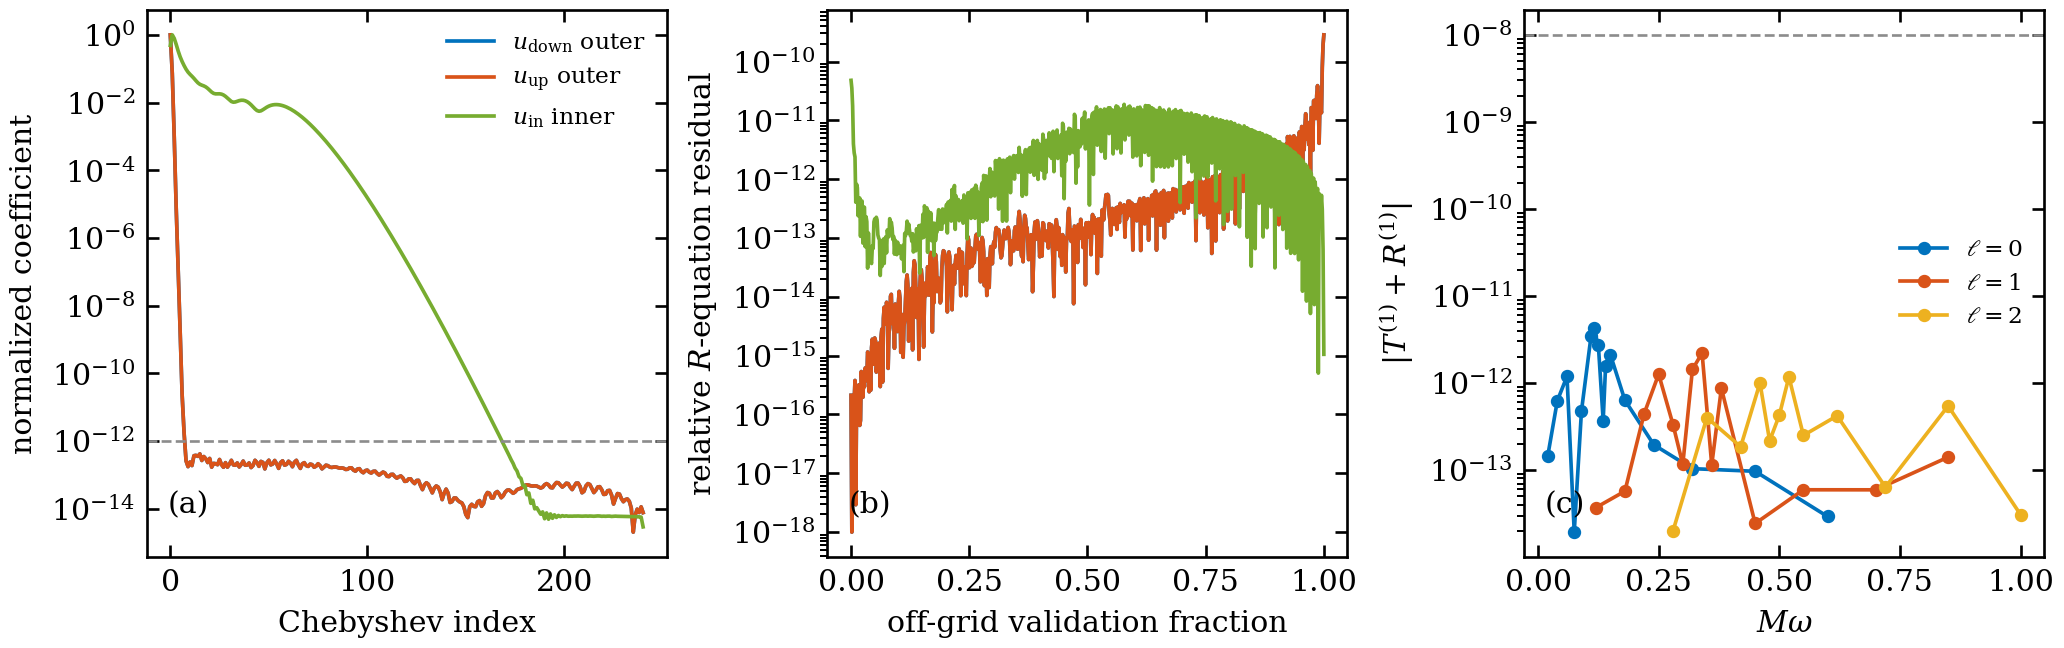
\includegraphics[width=0.95\textwidth]{../../figures/kerr_scalar_axisymmetric_accuracy.png}
\caption{Internal numerical accuracy diagnostics for the axisymmetric Kerr
calculation.  Panels (a) and (b) use the representative peak point
$a=0.5$, $m=0$, $\ell=2$, and $M\omega=0.52$ with $N=240$ and quadrature order
$q=192$.  Panel (a) shows the normalized Chebyshev coefficients of the
phase-peeled homogeneous solutions on the outer and inner subdomains.  Panel
(b) shows the relative residual \eqref{eq:radial_residual} after evaluating the
spectral interpolant and its analytic derivatives on 600 off-grid
Chebyshev--Gauss points per branch in the original radial Teukolsky equation.
Panel (c) shows the first-order flux-balance residual for the retained
axisymmetric points.  The dashed line marks the acceptance threshold
$10^{-8}$ used before any point enters the manuscript figures or fits.}
\label{fig:accuracy}
\end{figure*}

\subsection{Resonance and high-frequency diagnostics}
\label{sec:frequency-diagnostics}

The nonlinear boundary amplitude combines the scattering Green function
and the frequency-dependent source.  Write the cubic self-channel
coefficient as $A_H^{(1)}=-\mathcal I_H/W$, with
$\mathcal I_H=\int_{r_+}^\infty R^{\rm up}Q_{\ell\ell m}\,dr$.
The QNM frequencies are zeros of the analytically continued homogeneous
Wronskian.  On the real axis, the flux response also contains the source
projection, its phase, and the fixed-incident normalization in
Eq.~\eqref{eq:T1}.  This structure motivates a Breit--Wigner-type
description of a resolved peak and allows its center to shift relative to
the QNM real part.  We measure the peak position and width from the flux
curve and assess their stability under changes of the fitting window.

For the high-frequency analysis, the real scalar radial operator at real
$\omega>0$ gives $R^{\rm down}=\overline{R^{\rm up}}$ and
\begin{align}
R^{\rm in}&=B^{\rm inc}\overline{R^{\rm up}}+B^{\rm ref}R^{\rm up},
\nonumber\\
W&=2i\omega B^{\rm inc}.
\end{align}
Let $P(r)=r^2C^{(0)}_{\ell\ell m}+a^2C^{(2)}_{\ell\ell m}$, which is real,
and define the source projections
\begin{align}
J_{\rm d}&=\int_{r_+}^\infty P|R^{\rm in}|^2|R^{\rm up}|^2\,dr,
\nonumber\\
J_{\rm o}&=\int_{r_+}^\infty P|R^{\rm in}|^2(R^{\rm up})^2\,dr.
\end{align}
Substitution into the Green integral gives the exact decomposition
\begin{align}
A_H^{(1)}&=-\frac{1}{2i\omega}
\left[J_{\rm d}+\frac{B^{\rm ref}}{B^{\rm inc}}J_{\rm o}\right],
\nonumber\\
\chi_H&=-\frac{\operatorname{Im}[(B^{\rm ref}/B^{\rm inc})J_{\rm o}]}
{\omega|B^{\rm inc}|^2}.
\label{eq:kerr-tail-decomposition}
\end{align}
The real integral $J_{\rm d}$ contributes a horizon-phase shift.  The
absorbed-flux correction is the interference projection involving the
linear reflection amplitude and the oscillatory integral $J_{\rm o}$.
Thus its tail depends on their combined magnitude and relative phase.
This is the Kerr counterpart of the decomposition in Sec.~III.B.3 of the
Schwarzschild reference\cite{HeTianZhangManuscript2026}, with the Kerr
radial functions and covariant weight retained explicitly.

For the cubic Schwarzschild calculation, that reference obtains a
high-frequency envelope proportional to
$(M\omega)^{-1/2}\exp(-\omega/T_H)$ in its stated normalization and
source-sign convention.  This motivates testing
\begin{equation}
T^{(1)}_\ell\simeq A_\ell(M\omega)^{-\alpha}
\exp(-\omega/T_{\rm fit}),\qquad \alpha=0,\tfrac12,
\label{eq:tail-prefactor-model}
\end{equation}
on the same resolved Kerr samples.  The Kerr decay exponent requires
control of both factors in Eq.~\eqref{eq:kerr-tail-decomposition} and their
complex-radial continuation.  The available real-frequency calculations
test the finite-window models and their predictive residuals.

At high frequencies the phase-peeled homogeneous amplitudes become slowly
varying, while the nonlinear Green integral is controlled by rapidly
oscillatory tails.  Motivated by the thermal scale associated with a black-hole
horizon~\cite{Hawking1975} and by finite-window Boltzmann diagnostics in the
Kerr graybody-factor literature~\cite{Oshita2023,Oshita2024},
we test an exponential finite-window diagnostic using the Kerr radial
normalization and the $\Sigma$-weighted source.  The baseline model is
\begin{equation}
T_\ell^{(1)}(\omega)\simeq
A_\ell\exp\left[-\frac{\omega}{T_{\rm fit}}\right],
\qquad
\omega>\operatorname{Re}\omega_{\ell0}.
\label{eq:boltzmann}
\end{equation}
For Kerr
\begin{equation}
T_H=\frac{\rp-\rmn}{4\pi(\rp^2+a^2)}.
\end{equation}
For $a=0.5$ the fits in Sec.~\ref{sec:results} give
$\pi M T_{\rm fit}=0.111$, $0.105$, and $0.101$ for
$\ell=0,1,2$, close to $\pi M T_H=0.1160$.  These values should be read as
finite-window effective temperatures.  Their dependence on an algebraic
prefactor is tested in Sec.~\ref{sec:tail-results}.


\section{Results}
\label{sec:results}
\subsection{Resonant cubic response and the post-resonance tail}
\label{sec:resonance-results}
The finite-frequency cubic response is shown in
Fig.~\ref{fig:mainresults}.  It plots $T_\ell^{(1)}$ for $\ell=0,1,2$, uses a
linear scale to display the resonance peaks, and uses a logarithmic scale to
display the high-frequency tail.  The dashed lines mark the real parts of the
fundamental scalar Kerr quasinormal modes computed with the local
\texttt{qnm} package~\cite{Stein2019} for $s=0$, $a=0.5$, $m=0$, and $n=0$.

Three features are robust in the accepted data.  First, in the axisymmetric
Kerr cases studied here, $T_\ell^{(1)}$ is positive at every accepted sampled
frequency in the present flux
convention.  For positive coupling in Eq.~\eqref{eq:nonlinear_equation}, the
nonlinear correction therefore increases the absorbed flux and, by
Eq.~\eqref{eq:first_order_balance}, decreases the reflected flux at the same
order.  This sign statement refers to the coefficient convention of
Eqs.~\eqref{eq:T1} and \eqref{eq:R1}; it should not be compared to a reduced
Schwarzschild field convention without translating the flux normalization.

\subsubsection{Peak locations and source-weighted resonance}

The peaks of $T_\ell^{(1)}$ lie on the frequency scale set by the real
parts of the corresponding fundamental Kerr scalar QNMs~\cite{Berti2009,Stein2019}.  The fitted peak
positions are $M\omega_{\rm peak}=0.1306$, $0.3101$, and $0.5026$ for
$\ell=0,1,2$, while the QNM real parts are $0.1124$, $0.2979$, and $0.4920$.
The corresponding fractional offsets are $16.2\%$, $4.1\%$, and
$2.2\%$.
We characterize the real-frequency resonance by fitting the selected
samples to the four-parameter profile
\begin{equation}
T_\ell^{(1)}(\omega)=T_{\rm off}+
\frac{A\,\gamma^2}{(M\omega-\omega_p)^2+\gamma^2} .
\label{eq:lorentzian}
\end{equation}
Here $\omega_p$ is the fitted center in units $M=1$, and $\gamma$ is the
half-width parameter of the phenomenological Breit--Wigner-type interpolation.
The coefficient of determination of the three fits is $R^2=0.9918$,
$0.9978$, and $0.9985$ for $\ell=0,1,2$, respectively.
Equation~\eqref{eq:kerr-tail-decomposition} and the full Green integral
identify the flux as a source-weighted interference response.
Its fitted peak samples the QNM frequency scale together with the
frequency dependence of the nonlinear source and incident normalization.
A complex-frequency QNM projection requires a conserved bilinear form
and contour regularization~\cite{GreenEtAl2023}.
The fit uses the sampled points satisfying $T_\ell^{(1)}>0.2T_{\ell,\max}^{(1)}$;
the relative RMS residuals of these peak fits over the selected points are
$2.41\%$, $1.27\%$, and $1.05\%$ for $\ell=0,1,2$, respectively.  These
residuals quantify the descriptive quality of the real-frequency interpolation.
As a fit-window sensitivity check, we repeat the selection with thresholds
from $0.15$ to $0.30$ of the sampled maximum, retaining at least five points
in every fit.  The resulting fitted centers vary by at most
$6.7\times10^{-4}$, $3.9\times10^{-4}$, and $3.4\times10^{-4}$ for
$\ell=0,1,2$, respectively, whereas the corresponding half-widths vary by
$3.1\times10^{-3}$, $4.8\times10^{-3}$, and $5.2\times10^{-3}$.  The
center locations are therefore stable at the resolution of the sweep, while
the widths should be regarded as descriptive fit parameters.  The complete
threshold scan is included in the reproducibility data.

\subsubsection{High-frequency decay and its effective scale}
\label{sec:tail-results}

At high frequency the accepted tail points are well fit by the
Boltzmann form Eq.~\eqref{eq:boltzmann}.  The fitted temperatures differ from
the Kerr Hawking temperature by $4.0\%$, $9.8\%$, and $12.8\%$ for
$\ell=0,1,2$, respectively.  These are effective finite-window fit
parameters within the stated post-resonance windows.  On the accepted
low-frequency side the Kerr fixed-incident coefficients decrease as
$\omega$ is lowered over the globally balanced windows.  The deeper
horizon-side data then recover the matched Kerr powers $(M\omega)^{2\ell+2}$
with free-fit $R^2>0.999989$.  The comparison uses the fixed-incident normalization; the translation to
the reduced Schwarzschild convention is given in Appendix~\ref{app:flux}.

\begin{figure*}[t]
\centering
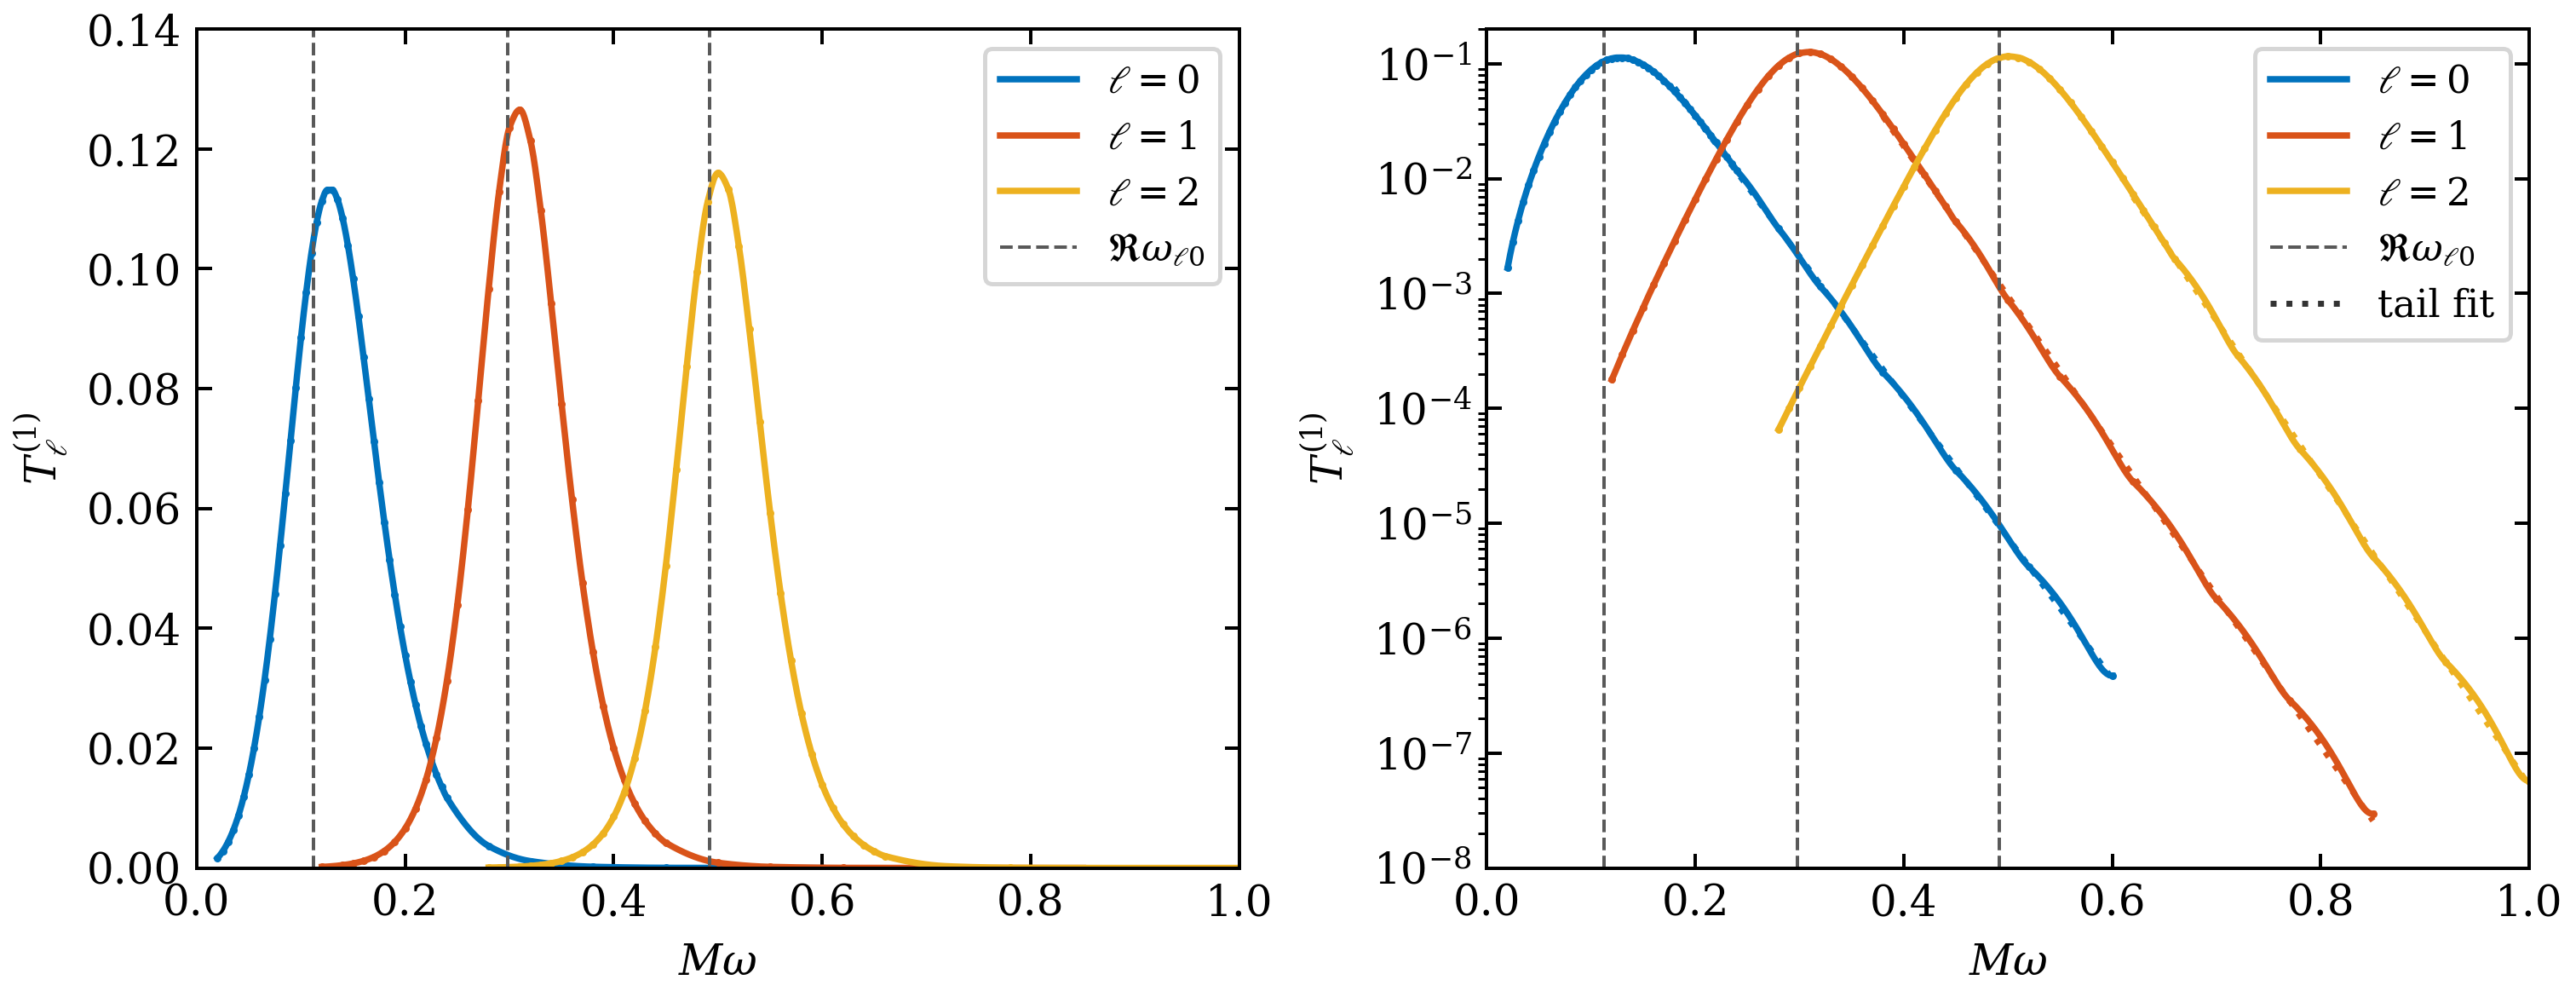
\includegraphics[width=0.92\textwidth]{../../figures/kerr_scalar_nonlinear_axisymmetric_fig2.png}
\caption{Nonlinear Kerr transmission coefficients
$T_\ell^{(1)}$ for $a=0.5$, $m=0$, and $\ell=0,1,2$.  The left panel uses a
linear scale to show the Breit--Wigner-type peaks.  The right panel uses a
logarithmic scale to show the exponential high-frequency tails; dotted
segments show the finite-window fits used in Table~\ref{tab:fit}.  Dashed
vertical lines mark the real parts of the fundamental scalar Kerr QNMs
$\operatorname{Re}\omega_{\ell0}$.  All 43 points entering the three tail-fit
windows use $q=2048$; the denser low-frequency and peak samples use $q=192$.
Circles show every accepted sample, while the solid curves are
shape-preserving interpolants used only as visual guides.  Every plotted point satisfies
$|T^{(1)}+R^{(1)}|\leq10^{-8}$.}
\label{fig:mainresults}
\end{figure*}

\begin{table}[t]
\caption{Fitting parameters of the Kerr nonlinear transmission resonance and
the high-frequency Boltzmann tail.  The QNM frequencies are scalar Kerr
fundamental modes with $s=0$, $a=0.5$, $m=0$, and $n=0$.  All frequencies are
reported in units $M=1$.}
\label{tab:fit}
\begin{ruledtabular}
\begin{tabular}{c c c c c c c}
$\ell$ & $\omega_p$ & $\gamma$
& $\Re\omega_Q$
& $|\Im\omega_Q|$
& $\pi T_{\rm fit}$
& $\Delta T$\\
\hline
0 & 0.1306 & 0.0599 & 0.1124 & 0.1022 & 0.1114 & 4.00\%\\
1 & 0.3101 & 0.0591 & 0.2979 & 0.0954 & 0.1046 & 9.85\%\\
2 & 0.5026 & 0.0595 & 0.4920 & 0.0946 & 0.1012 & 12.81\%\\
\end{tabular}
\end{ruledtabular}
\end{table}

The exponential fits use unweighted least squares for
$\log T_\ell^{(1)}$ versus $M\omega$ over the windows
$[0.18,0.60]$, $[0.38,0.85]$, and $[0.62,1.00]$ for
$\ell=0,1,2$, respectively.  The corresponding root-mean-square residuals
in log space are $3.7\times10^{-2}$, $6.7\times10^{-2}$, and
$5.6\times10^{-2}$.  These window-dependent residuals quantify the quality
of the finite-window fit; they are not estimates of a systematic error outside
the computed frequency range.

Because the effective temperature is a fit diagnostic rather than an analytic
observable, we also repeat the tail fit after shifting either edge of each
window while retaining at least three positive data points.  The resulting
window ranges and the largest logarithmic fit residual are given in
Table~\ref{tab:tail-window}.  The fitted values vary only at the percent level
within these local windows, while their absolute offsets from $T_H$ remain
consistent with the finite-window qualification above.

\begin{table*}[t]
\caption{Sensitivity of the finite-window effective temperatures to the fit
window.  The baseline window is the one used in Table~\ref{tab:fit}; the range
is obtained from three nearby edge-shifted windows.  The final column is the
largest absolute fractional offset from the Kerr Hawking temperature among
the four windows.}
\label{tab:tail-window}
\begin{ruledtabular}
\begin{tabular}{c c c c c c}
$\ell$ & baseline $[M\omega_{\min},M\omega_{\max}]$
& $\pi T_{\rm fit}^{\rm base}$ & range of $\pi T_{\rm fit}$
& $\max\sigma_{\log}$ & $\max|T_{\rm fit}/T_H-1|$\\
\hline
0 & $[0.18,0.60]$ & 0.1114 & $[0.1109,0.1122]$ & $3.86\times10^{-2}$ & 4.45\%\\
1 & $[0.38,0.85]$ & 0.1046 & $[0.1037,0.1068]$ & $6.95\times10^{-2}$ & 10.61\%\\
2 & $[0.62,1.00]$ & 0.1012 & $[0.1002,0.1031]$ & $5.59\times10^{-2}$ & 13.62\%\\
\end{tabular}
\end{ruledtabular}
\end{table*}

To test whether a power law can mimic the exponential over these finite
windows, we fit the same positive data to
$\log T^{(1)}=c-\beta M\omega$ and
$\log T^{(1)}=c-n\log(M\omega)$.  Both models have two fitted parameters, so
their corrected Akaike information criteria can be compared without a
parameter-count ambiguity.  For $n_s$ samples and $k=2$ fitted parameters we
use
\begin{equation}
\mathrm{AICc}=n_s\log(\mathrm{RSS}/n_s)+2k
+\frac{2k(k+1)}{n_s-k-1},
\label{eq:aicc}
\end{equation}
with the residual sum of squares evaluated in log space.
Table~\ref{tab:tail-models} also reports
leave-one-out prediction residuals.  The exponential has the smaller AICc and
the smaller predictive residual for every $\ell$.  A fit with the exponential
slope fixed exactly to $-1/T_H$ has logarithmic RMS residuals $0.139$, $0.443$,
and $0.514$ for $\ell=0,1,2$; hence the data support a finite-window
exponential more strongly than either a power law or an exact thermal slope.
This comparison establishes exponential decay as the preferred description
within the resolved windows.  Extending the frequency interval tests its
asymptotic persistence.

\subsubsection{Algebraic prefactor and the Schwarzschild comparison}

We next fit Eq.~\eqref{eq:tail-prefactor-model} with $\alpha=1/2$ to the
same $19,14,10$ samples used by the baseline exponential.
Both models have two fitted parameters, the amplitude and the decay scale.
Table~\ref{tab:tail-prefactor20261014} reports their logarithmic residuals,
leave-one-out prediction errors, and AICc differences.  The prefactor
improves the residuals for $\ell=1,2$, with the stronger preference at
$\ell=1$; for $\ell=0$ the baseline exponential has the smaller AICc and
the two predictive errors are nearly equal.  These channel-dependent
comparisons quantify how an algebraic factor changes the decay scale
in the measured finite-frequency regime.

\begin{table*}[t]
\caption{Schwarzschild-inspired prefactor test on the same Kerr tail
windows as Table~\ref{tab:tail-models}.  The fitted model is
$A(M\omega)^{-1/2}\exp(-\omega/T_{1/2})$.
$\Delta\mathrm{AICc}=\mathrm{AICc}_{1/2}-\mathrm{AICc}_{\rm exp}$;
negative values favor the prefactor model.  The last column fixes its
temperature to the Kerr $T_H$ and fits the amplitude alone.  All residuals
are RMS errors in $\log T^{(1)}$.}
\label{tab:tail-prefactor20261014}
\begin{ruledtabular}
\begin{tabular}{cccccc}
$\ell$ & $\pi MT_{1/2}$ & $\sigma_{1/2}$ &
$\sigma_{\rm LOO,1/2}$ & $\Delta\mathrm{AICc}$ & $\sigma_{1/2,T_H}$\\
\hline
0 & 0.11754 & 0.04186 & 0.04572 & $+4.48$ & 0.05893\\
1 & 0.10772 & 0.05505 & 0.07332 & $-5.53$ & 0.31412\\
2 & 0.10328 & 0.05094 & 0.07388 & $-1.85$ & 0.43161\\
\end{tabular}
\end{ruledtabular}
\end{table*}

The logarithmic slope of the prefactor model satisfies
\begin{equation}
-\frac{d\log T^{(1)}}{d\omega}
=\frac{1}{T_{\rm fit}}+\frac{\alpha}{\omega}.
\label{eq:tail-effective-slope}
\end{equation}
A pure exponential fit therefore incorporates the algebraic contribution
into its effective inverse temperature.  Including $\alpha=1/2$ raises
$\pi MT_{\rm fit}$ from $0.11139,0.10460,0.10116$ to
$0.11754,0.10772,0.10328$ for $\ell=0,1,2$.  The revised scale lies within
$1.3\%$ of $T_H$ for the monopole.  The exact-$T_H$ prefactor model has
RMS residuals $0.05893,0.31412,0.43161$; the free-scale model resolves the
remaining modal dependence.  The source weight, reflection amplitude,
and phase in Eq.~\eqref{eq:kerr-tail-decomposition} supply the quantities
whose high-frequency asymptotics determine that dependence.  This connects
the numerical tail to the Schwarzschild analytic argument while retaining
the Kerr-specific ingredients.

\begin{table*}[t]
\caption{Finite-window comparison of exponential and power-law descriptions
of the high-frequency nonlinear transmission tail.  The residuals are RMS
errors in $\log T^{(1)}$; $\Delta\mathrm{AICc}$ is
$\mathrm{AICc}_{\rm power}-\mathrm{AICc}_{\rm exp}$, so positive values favor
the exponential.  The final two columns are leave-one-out logarithmic
prediction residuals.}
\label{tab:tail-models}
\begin{ruledtabular}
\begin{tabular}{c c c c c c c}
$\ell$ & points & $\sigma_{\rm exp}$ & $\sigma_{\rm power}$
& $\Delta\mathrm{AICc}$ & $\sigma_{\rm LOO,exp}$ & $\sigma_{\rm LOO,power}$\\
\hline
0 & 19 & $3.72\times10^{-2}$ & $4.89\times10^{-1}$ & 97.9 & $4.56\times10^{-2}$ & $6.09\times10^{-1}$\\
1 & 14 & $6.71\times10^{-2}$ & $3.75\times10^{-1}$ & 48.2 & $8.92\times10^{-2}$ & $4.80\times10^{-1}$\\
2 & 10 & $5.59\times10^{-2}$ & $1.84\times10^{-1}$ & 23.8 & $8.11\times10^{-2}$ & $2.62\times10^{-1}$\\
\end{tabular}
\end{ruledtabular}
\end{table*}

All peak and tail fits, and all filled sweep points in
Figs.~\ref{fig:lowfreq} and \ref{fig:mainresults}, use only the accepted
globally balanced subset.  The open infrared points in
Fig.~\ref{fig:lowfreq} instead obey the paired horizon-side and Wronskian
checks stated above.  The largest first-order balance residual of the global
subset
is $6.9\times10^{-12}$, $2.2\times10^{-12}$, and
$1.5\times10^{-12}$ for $\ell=0,1,2$, respectively.  Completed solver rows
that fail the $10^{-8}$ gate remain in the reproducibility data as an audit
trail, but they are omitted from the plots, tables, peak interpolation, and
low-frequency discussion.  No physical claim is based on those excluded rows.

\begin{table*}[t]
\caption{Numerical quality of the axisymmetric Kerr frequency sweeps.  Here
$\delta_0=|T^{(0)}+R^{(0)}-1|$ and
$\delta_1=|T^{(1)}+R^{(1)}|$.  Every retained point satisfies
$\delta_1\le 10^{-8}$.  All active points use $N=240$.  The low-frequency and
peak samples use $q=192$.  All 43 samples in the three tail-fit windows use
$q=2048$ after the audit in Table~\ref{tab:tail-convergence}.  The earlier
$N=224$, $q=160$ peak sweep is retained as the production-resolution audit in
Table~\ref{tab:production-convergence}.  The final column is the
root-mean-square residual of the logarithmic high-frequency tail fit.}
\label{tab:numerics}
\begin{ruledtabular}
\begin{tabular}{c c c c c c}
$\ell$ & retained & $M\omega_{\min}$ & $\max\delta_0$ & $\max\delta_1$
& $\sigma_{\rm tail}$\\
\hline
0 & 51 & 0.02 & $2.8\times10^{-11}$ & $6.9\times10^{-12}$ & $3.7\times10^{-2}$\\
1 & 40 & 0.12 & $1.9\times10^{-11}$ & $2.2\times10^{-12}$ & $6.7\times10^{-2}$\\
2 & 44 & 0.28 & $3.8\times10^{-11}$ & $1.5\times10^{-12}$ & $5.6\times10^{-2}$\\
\end{tabular}
\end{ruledtabular}
\end{table*}

The change from the former production resolution to the active refined
resolution is quantified separately in Table~\ref{tab:production-convergence}.
At the representative peak points the refined calculation changes the
transmission coefficient by at most $3.2\times10^{-5}$ and preserves the
first-order flux balance at the $10^{-12}$ level.  We therefore use the
refined curves for the physical discussion below; the lower-resolution values
are reported to make the resolution choice auditable rather than folded into
an unreported systematic error.

\begin{table*}[t]
\caption{Production-resolution audit for the axisymmetric Kerr calculation.
The entries compare the former production configuration $(N,q)=(224,160)$
with the active reference configuration $(N,q)=(240,192)$ at fixed
$r_{\rm m}=40$.  Each entry in the first four columns is
$|X_{240,192}-X_{224,160}|/|X_{240,192}|$ for the indicated Green-function
amplitude or flux coefficient; the final column is the
absolute first-order balance residual of the reference run.}
\label{tab:production-convergence}
\begin{ruledtabular}
\begin{tabular}{c c c c c c}
case & $\Delta A_{\rm ref}$ & $\Delta A_H$
& $\Delta T^{(1)}$ & $\Delta R^{(1)}$ & $|\delta_1|_{\rm ref}$\\
\hline
$\ell=0,\ M\omega=.125$ & $4.5\times10^{-7}$ & $7.8\times10^{-7}$
& $2.3\times10^{-6}$ & $2.3\times10^{-6}$ & $2.7\times10^{-12}$\\
$\ell=1,\ M\omega=.34$ & $5.9\times10^{-6}$ & $3.3\times10^{-6}$
& $1.5\times10^{-5}$ & $1.5\times10^{-5}$ & $2.2\times10^{-12}$\\
$\ell=2,\ M\omega=.52$ & $9.6\times10^{-6}$ & $7.6\times10^{-6}$
& $3.1\times10^{-5}$ & $3.1\times10^{-5}$ & $1.2\times10^{-12}$\\
\end{tabular}
\end{ruledtabular}
\end{table*}

The high-frequency tail requires a separate quadrature audit because flux
balance alone does not detect a common error in the two interference terms.
At fixed $N=240$, the compact inner integral was scanned from $q=192$ to
$q=2048$, with twelve intermediate orders, at the three representative points
in Table~\ref{tab:tail-convergence}.  The sequence
is mildly nonmonotonic at intermediate order but reaches a plateau at the two
largest orders.  We therefore recomputed every point entering the tail fits at
$q=2048$.  Lowering $N$ at fixed $q=2048$ produces a much smaller change,
showing that the remaining sensitivity belongs to the oscillatory Green
integral rather than to the homogeneous spectral solution.

\begin{table*}[t]
\caption{High-frequency convergence audit for the active tail data.  The
quadrature columns compare $q=1792$ with the $q=2048$ reference at $N=240$;
the radial-order column compares $N=224$ with $N=240$ at $q=2048$.  All
entries except the final balance residual are relative changes with respect to
the reference.}
\label{tab:tail-convergence}
\begin{ruledtabular}
\begin{tabular}{c c c c c c}
case & $\Delta T^{(1)}[q]$ & $\Delta T^{(1)}[N]$
& $\Delta A_{\rm ref}[q]$ & $\Delta A_H[q]$ & $|\delta_1|_{\rm ref}$\\
\hline
$\ell=0,\ M\omega=.52$ & $3.0\times10^{-5}$ & $7.1\times10^{-10}$ & $2.3\times10^{-5}$ & $1.6\times10^{-9}$ & $7.8\times10^{-15}$\\
$\ell=1,\ M\omega=.77$ & $1.7\times10^{-4}$ & $1.0\times10^{-9}$ & $3.1\times10^{-4}$ & $1.2\times10^{-9}$ & $2.7\times10^{-13}$\\
$\ell=2,\ M\omega=.92$ & $2.5\times10^{-4}$ & $9.5\times10^{-8}$ & $3.4\times10^{-4}$ & $2.5\times10^{-9}$ & $1.0\times10^{-14}$\\
\end{tabular}
\end{ruledtabular}
\end{table*}

\subsection{Infrared response and local-power hierarchy}

The scalar monopole provides an analytic low-frequency normalization check
directly in the Kerr Teukolsky variable.  Fix $|a|<M$, take
$(\ell,m)=(0,0)$, and introduce the far-zone coordinate $x=\omega r$.
In the limit $\omega\to0$ the normalized spheroidal harmonic and the
self-channel projector become
\begin{equation}
 S_{00}\longrightarrow\frac{1}{\sqrt{4\pi}},\qquad
 C^{(0)}_{000}\longrightarrow\frac{1}{4\pi}.
 \label{eq:l0-angular-limit}
\end{equation}
The leading far-zone radial equation is the flat-space monopole equation.
Matching to the solution that is unity at the horizon gives
\begin{align}
 R^{\rm in}_{00\omega}
 &=j_0(x)+o(1)=\frac{\sin x}{x}+o(1),\nonumber\\
 R^{\rm up}_{00\omega}
 &=\frac{e^{\ii x}}{r}[1+o(1)].
 \label{eq:l0-far-solutions}
\end{align}
Comparison with Eq.~\eqref{eq:bc_inf} and evaluation of
Eq.~\eqref{eq:wronskian} at infinity then yield
\begin{equation}
 B^{\rm inc}_{00\omega}=\frac{\ii}{2\omega}[1+o(1)],
 \qquad
 W_0=2\ii\omega B^{\rm inc}_{00\omega}=-1+o(1).
 \label{eq:l0-binc-wronskian}
\end{equation}

The $a^2C^{(2)}$ part of the source and all strong-field corrections are
subleading relative to the far-zone $r^2C^{(0)}$ term.  Substitution of
Eqs.~\eqref{eq:l0-angular-limit}--\eqref{eq:l0-binc-wronskian} into the
horizon Green integral therefore gives the full complex amplitude
\begin{align}
 A_{H,00}^{(1)}
 &=\frac{C^{(0)}_{000}}{\omega^2}
 \int_0^\infty\frac{\sin^3x\,e^{\ii x}}{x^2}\,\dd x
 +o(\omega^{-2})\nonumber\\
 &=\frac{C^{(0)}_{000}}{\omega^2}(I_0+\ii J_0)
 +o(\omega^{-2}),
 \label{eq:l0-green-limit}
\end{align}
where both integrals can be evaluated without a regulator.  Using
$\sin^3x\cos x=\tfrac14\sin 2x-\tfrac18\sin4x$ and integrating by parts,
\begin{equation}
 \begin{split}
 I_0&=\int_0^\infty\frac{\sin^3x\cos x}{x^2}\,\dd x\\
 &=\frac12\int_0^\infty\frac{\cos2x-\cos4x}{x}\,\dd x
 =\frac12\ln2 .
\end{split}
\label{eq:l0-integral}
\end{equation}
while a second integration by parts gives
\begin{equation}
 J_0=\int_0^\infty\frac{\sin^4x}{x^2}\,\dd x
 =4\int_0^\infty\frac{\sin^3x\cos x}{x}\,\dd x
 =\frac{\pi}{4}.
 \label{eq:l0-phase-integral}
\end{equation}
Since $C^{(0)}_{000}=1/(4\pi)$, the amplitude and relative response are
\begin{align}
 A_{H,00}^{(1)}
 &=\left(\frac{\ln2}{8\pi}+\frac{\ii}{16}\right)\omega^{-2}
 +o(\omega^{-2}),\nonumber\\
 \rho_{H,00}
 &\longrightarrow\frac{\ln2}{2\pi}+\frac{\ii}{4}.
 \label{eq:l0-complex-response}
\end{align}
The imaginary term is a finite horizon phase response after incident
normalization; it does not contribute to the first-order energy flux.  The
real part and Eq.~\eqref{eq:horizon_response} give
\begin{equation}
 \boxed{\displaystyle
 \lim_{\omega\to0}\chi_{H,00}
 =8C^{(0)}_{000}I_0
 =\frac{\ln 2}{\pi}=0.220635600153 .}
 \label{eq:l0-exact-response}
\end{equation}
The leading result is independent of spin because the limit is controlled by
the far zone.  The closed form $\ln2/\pi$ is specific to the scalar monopole
and is not a superradiant-threshold result: $m=0$ implies $p=\omega$.

The same matching argument determines both absolute flux coefficients for
every cubic axisymmetric self channel.  Let
$d=(M^2-a^2)^{1/2}$ and first set $\omega=0$.  The horizon-regular radial
equation and its unit-horizon solution are
\begin{equation}
 \frac{\dd}{\dd r}\left(\DeltaK\frac{\dd R}{\dd r}\right)
 -\ell(\ell+1)R=0,
 \qquad
 R=P_\ell\!\left(\frac{r-M}{d}\right),
 \label{eq:axisymmetric-static-solution}
\end{equation}
because $P_\ell(1)=1$.  Since the leading coefficient of $P_\ell(z)$ is
$q_\ell=(2\ell)!/[2^\ell(\ell!)^2]$, matching the growing part of
Eq.~\eqref{eq:axisymmetric-static-solution} to the small-$x$ limit of
$j_\ell(x)$ gives
\begin{align}
 R^{\rm in}_{\ell0\omega}
 &= {\cal K}_\ell(M\omega)^{-\ell}j_\ell(x)[1+o(1)],\nonumber\\
 {\cal K}_\ell
 &=(2\ell+1)!!\,q_\ell\left(\frac{M}{d}\right)^\ell,
 \qquad x=\omega r .
 \label{eq:axisymmetric-far-match}
\end{align}
The incoming part of $j_\ell$ fixes both the phase and magnitude,
\begin{align}
 B^{\rm inc}_{\ell0\omega}
 &=\frac{M\ii^{\ell+1}{\cal K}_\ell}
 {2(M\omega)^{\ell+1}}[1+o(1)],\nonumber\\
 |B^{\rm inc}_{\ell0\omega}|^2
 &=\frac{M^2{\cal K}_\ell^2}
 {4(M\omega)^{2\ell+2}}[1+o(1)].
 \label{eq:axisymmetric-binc-limit}
\end{align}
Substitution into Eq.~\eqref{eq:linear_coefficients}, with $p=\omega$, yields
the absolute linear law
\begin{align}
 T^{(0)}_{\ell0}
 &={\cal A}^{(0)}_\ell(M\omega)^{2\ell+2}[1+o(1)],\nonumber\\
 {\cal A}^{(0)}_\ell
 &=\frac{4(r_+^2+a^2)}{M^2{\cal K}_\ell^2}.
 \label{eq:axisymmetric-T0-infrared}
\end{align}

For the nonlinear coefficient, define the spherical angular overlap and two
convergent Bessel integrals
\begin{align}
 {\cal C}_\ell=\int|Y_{\ell0}|^4\dd\Omega,
 \qquad &
 {\cal I}_\ell=-\int_0^\infty x^2y_\ell(x)j_\ell^3(x)\dd x ,\nonumber\\
 &{\cal J}_\ell=\int_0^\infty x^2j_\ell^4(x)\dd x>0.
 \label{eq:axisymmetric-infrared-integral}
\end{align}
For fixed subextremal spin the $a^2C^{(2)}$ source term and the strong-field
part of the Green integral are subleading.  In units $M=1$, the outgoing
solution and Wronskian in the far zone are
$R^{\rm up}=\omega\ii^{\ell+1}h_\ell^{(1)}(x)[1+o(1)]$ and
$W_\ell=\ii^{\ell+2}{\cal K}_\ell\omega^{-\ell}[1+o(1)]$.
Their phases are essential.  Since
$\ii h_\ell^{(1)}=\ii j_\ell-y_\ell$, direct substitution in the Green
integral gives, after restoring $M$,
\begin{equation}
 \frac{A_{H,\ell0}^{(1)}}{M^2}
 ={\cal C}_\ell{\cal K}_\ell^2
 ({\cal I}_\ell+\ii{\cal J}_\ell)
 (M\omega)^{-2\ell-2}[1+o(1)].
 \label{eq:axisymmetric-AH-infrared}
\end{equation}
Thus the unit-horizon coefficient has
$|A_H^{(1)}|\propto(M\omega)^{-2\ell-2}$ and
$\arg A_H^{(1)}\to\arg({\cal I}_\ell+\ii{\cal J}_\ell)$.  This divergence is
not a divergent scattering response: maintaining unit horizon amplitude
requires a growing incident wave as $\omega\to0$.  Combining
Eqs.~\eqref{eq:axisymmetric-binc-limit} and
\eqref{eq:axisymmetric-AH-infrared} instead gives
\begin{align}
 M A_{H,{\rm fix}}^{(1)}
 &=\frac{8{\cal C}_\ell}{{\cal K}_\ell}\ii^{-(\ell+1)}
 ({\cal I}_\ell+\ii{\cal J}_\ell)
 (M\omega)^{\ell+1}[1+o(1)],\nonumber\\
 \rho_{H,\ell0}
 &\longrightarrow\rho^{\rm IR}_{H,\ell}
 =4{\cal C}_\ell({\cal I}_\ell+\ii{\cal J}_\ell).
 \label{eq:axisymmetric-complex-response}
\end{align}
The fixed-incident first-order amplitude therefore vanishes as
$(M\omega)^{\ell+1}$, while its ratio to the linear horizon amplitude tends
to a finite complex constant.  Taking its real part cancels the near-zone
matching coefficient and recovers the flux laws
\begin{align}
 \chi_{H,\ell0}
 &\longrightarrow \chi^{\rm IR}_\ell
 =2\operatorname{Re}\rho^{\rm IR}_{H,\ell}
 =8{\cal C}_\ell{\cal I}_\ell,\nonumber\\
 T^{(1)}_{\ell0}
 &={\cal A}^{(1)}_\ell(M\omega)^{2\ell+2}[1+o(1)],
 \qquad
 {\cal A}^{(1)}_\ell={\cal A}^{(0)}_\ell\chi^{\rm IR}_\ell .
 \label{eq:axisymmetric-T1-infrared}
\end{align}
Thus the cubic fractional response is unsuppressed in the infrared for
every axisymmetric self channel: it changes the coefficient, but not the linear absorption
power.  The ratio $\chi^{\rm IR}_\ell$ is independent of spin, although the
absolute coefficients retain spin dependence through ${\cal K}_\ell$ and the
horizon-area factor.  This statement takes $\omega\to0$ at fixed $|a|<M$;
Eq.~\eqref{eq:axisymmetric-static-solution} also makes clear why the limit is
not uniform as $a/M\to1$ for $\ell>0$.

Table~\ref{tab:axisymmetric-infrared} evaluates the new formulas for the
$a/M=0.5$ production spin.  The Bessel integrals were summed over successive
$\pi$ intervals and extrapolated in inverse endpoint powers.  Independent
Kerr solves at $(N,q)=(144,144)$ and $(176,176)$ used only the horizon-side
response at the listed lowest frequencies.  At the higher resolution the
relative differences between the scaled numerical and analytic coefficients
are $(0.48,0.96,3.32)\%$ for $T^{(0)}$ and $(0.82,1.07,3.41)\%$ for
$T^{(1)}$, ordered by $\ell=0,1,2$; these are finite-frequency corrections,
not fitted exponents.  The two-resolution changes in $\chi_H$ are given in
the final column, and the largest Wronskian error is $2.5\times10^{-11}$.
The same runs test information absent from the energy flux.  For
$\ell=0,1,2$ they give
$\mathcal J_\ell=(0.785398163397,0.366519142919,0.246839422782)$ and limiting
phases $(66.1895^\circ,70.6933^\circ,72.4699^\circ)$.  At the lowest listed
frequencies the complex relative responses agree with
Eq.~\eqref{eq:axisymmetric-complex-response} to
$(0.228,0.148,0.318)\%$, while their simultaneous-resolution changes are
$(6.3\times10^{-6},5.0\times10^{-5},3.0\times10^{-4})$.  Hence both the
dissipative real part and the reactive phase part are independently resolved.
The infinity-side $R^{(1)}$ interference term is already cancellation limited
at these frequencies and is deliberately not used in this infrared audit.

As a numerical test of the powers rather than only their coefficients, we fit
the seven horizon-side points for each multipole freely in log--log space.
For $T^{(0)}$ the fitted powers are $2.0145$, $4.0298$, and $6.0784$; for
$T^{(1)}$ they are $2.0245$, $4.0360$, and $6.0884$.  Every fit has
$R^2>0.999989$.  Restricting to the lowest five frequencies moves the two
sets to $(2.0095,4.0193,6.0502)$ and $(2.0162,4.0237,6.0585)$,
respectively, showing convergence toward the exact powers $(2,4,6)$ as the
upper end of the fit window is removed.  The analytic conclusion still comes
from matched asymptotics; these free fits are an independent finite-frequency
audit.  For $\ell=2$, attempts at $M\omega=0.003$ and $0.004$ failed the
paired continuation-normalization check and are excluded, so the reported
infrared window begins at $M\omega=0.005$.

\begin{table*}[t]
\caption{Analytic cubic infrared coefficients and direct horizon-side checks
for $a/M=0.5$.  Here
$T^{(i)}_{\ell0}\sim{\cal A}^{(i)}_\ell(M\omega)^{2\ell+2}$ and
$\delta_N\chi_H$ compares the simultaneous $(N,q)=(144,144)$ and
$(176,176)$ calculations at the lowest listed frequency.}
\label{tab:axisymmetric-infrared}
\begin{ruledtabular}
\begin{tabular}{c c c c c c c}
$\ell$ & ${\cal I}_\ell$ & $\chi^{\rm IR}_\ell$
& ${\cal A}^{(0)}_\ell$ & ${\cal A}^{(1)}_\ell$
& lowest $M\omega$ & $\delta_N\chi_H$\\
\hline
0 & 0.346573590280 & 0.220635600153 & 14.9282032 & 3.29369308 & 0.00075 & $1.1\times10^{-7}$\\
1 & 0.128401008797 & 0.147136717786 & 1.24401694 & 0.183040569 & 0.00150 & $1.5\times10^{-4}$\\
2 & 0.077970747421 & 0.106366541731 & 0.0165868925 & 0.00176429039 & 0.00500 & $7.7\times10^{-5}$\\
\end{tabular}
\end{ruledtabular}
\end{table*}

This calculation extends analytically to every positive integer $n$.  Consider
the $U(1)$-invariant local equation
\begin{equation}
 \Box\Phi+\epsilon_n|\Phi|^{2n}\Phi=0,
 \qquad n=1,2,\ldots,
 \label{eq:power-nonlinearity}
\end{equation}
for which $[\epsilon_n]=M^{2n-2}$ when $[\Phi]=M^{-1}$.  The cubic model used
elsewhere in this paper is the $n=1$ member.  At first order the source scales
as $|\alpha|^{2n}\alpha$ under
$R^{(0)}\mapsto\alpha R^{(0)}$, so fixed-incident normalization gives
\begin{align}
 T_n^{(1)}&=\frac{2p(r_+^2+a^2)}{\omega|B^{\rm inc}|^{2n+2}}
 \operatorname{Re}A_{H,n}^{(1)},\nonumber\\
 \chi_H^{(n)}&\equiv\frac{T_n^{(1)}}{T^{(0)}}
 =\frac{2\operatorname{Re}A_{H,n}^{(1)}}{|B^{\rm inc}|^{2n}}.
 \label{eq:power-response}
\end{align}
For a general incident mode and target multipole the projected source is
\begin{align}
 Q^{(n)}_{\ell'\ell m}(r)={}&
 \left[r^2C^{(0,n)}_{\ell'\ell m}
 +a^2C^{(2,n)}_{\ell'\ell m}\right]
 |R^{\rm in}_{\ell m\omega}|^{2n}R^{\rm in}_{\ell m\omega},
 \label{eq:power-radial-source}\\
 C^{(j,n)}_{\ell'\ell m}={}&\int\dd\Omega\,\cos^j\theta\,
 S_{\ell'm}^*|S_{\ell m}|^{2n}S_{\ell m},
 \qquad j=0,2 .
 \label{eq:power-angular-general}
\end{align}
The Green amplitudes follow from the same in/up Wronskian as in the cubic
calculation, with $Q\mapsto Q^{(n)}$.  In particular,
\begin{equation}
 A_{H,n}^{(1)}=-\frac{1}{W_\ell}\int_{r_+}^{\infty}
 Q^{(n)}_{\ell\ell m}(r)R^{\rm up}_{\ell m\omega}(r)\dd r .
 \label{eq:power-horizon-green}
\end{equation}
For a dimensionless incident amplitude ${\cal A}_{\rm in}$, the self-channel
flux expansion and its conservation law are
\begin{align}
 T={}&T^{(0)}+\epsilon_n|{\cal A}_{\rm in}|^{2n}T_n^{(1)}
 +\calO(\epsilon_n^2|{\cal A}_{\rm in}|^{4n}),\nonumber\\
 R={}&R^{(0)}+\epsilon_n|{\cal A}_{\rm in}|^{2n}R_n^{(1)}
 +\calO(\epsilon_n^2|{\cal A}_{\rm in}|^{4n}),\nonumber\\
 T_n^{(1)}+R_n^{(1)}={}&0 .
 \label{eq:power-flux-expansion}
\end{align}
This makes $M^{2n-2}\chi_H^{(n)}$ dimensionless.  Numerically, the outer
integrand is not formed by raising a cancellation-prone oscillatory sum to a
large power.  We expand
$(B^{\rm inc}e^{-\ii\omega r_*}+B^{\rm ref}e^{\ii\omega r_*})^{n+1}$ and
its conjugate factor binomially, multiply by the target homogeneous wave, and
integrate the resulting finite phase channels separately.  This gives
$2n+3$ channels with phase indices
$q=-2n-2,-2n,\ldots,2n+2$ and asymptotic envelope $r^{-2n}$.
The construction is therefore finite for every fixed positive integer $n$
and retains oscillatory-tail control as the operator order is increased.

For the monopole the angular projections reduce to
\begin{equation}
 C_n^{(0)}=\int|S_{00}|^{2n+2}\dd\Omega=(4\pi)^{-n},
 \qquad C_n^{(2)}=\frac13C_n^{(0)}.
 \label{eq:power-angular}
\end{equation}
The leading far-zone Green integral is consequently
\begin{align}
 \operatorname{Re}A_{H,n}^{(1)}
 &=\frac{C_n^{(0)}}{\omega^2}I_n+o(\omega^{-2}),\nonumber\\
 I_n&=\int_0^\infty
 \frac{\sin^{2n+1}x\cos x}{x^{2n}}\dd x,\nonumber\\
 &=\frac{n}{n+1}\int_0^\infty
 \frac{\sin^{2n+2}x}{x^{2n+1}}\dd x>0.
 \label{eq:power-integral}
\end{align}
The second form follows by integration by parts and proves positivity without
numerics.  Repeated integration by parts, followed by the standard finite
cosine expansion of $\sin^{2n+2}x$, gives the regulator-independent finite sum
\begin{equation}
 I_n=\frac{(-1)^n}{4(n+1)(2n-1)!}
 \sum_{j=1}^{n+1}(-1)^{j+1}j^{2n}
 \binom{2n+2}{n+1-j}\ln j .
 \label{eq:power-integral-sum}
\end{equation}
Using $B^{\rm inc}=\ii/(2\omega)+o(\omega^{-1})$ in
Eq.~\eqref{eq:power-response} yields the all-$n$ infrared law
\begin{align}
 M^{2n-2}\chi_{H,00}^{(n)}
 &=c_n(M\omega)^{2n-2}\nonumber\\
 &\quad+o\!\left((M\omega)^{2n-2}\right),
 \label{eq:power-infrared-law}\\
 c_n&=\frac{2I_n}{\pi^n}>0 .\nonumber
\end{align}
Thus $n=1$ retains a finite infrared response and reproduces
$c_1=\ln2/\pi$, whereas every $n>1$ interaction produces a
power-suppressed fractional response in this scattering observable.  The next two coefficients are
\begin{equation}
 c_2=0.0631722552062,\qquad c_3=0.0172436384309.
 \label{eq:power-coefficients}
\end{equation}

For the full $\ell=0,1,2$ spectra, the far-zone normalization and the
covariant source weight
$r^2C^{(0)}_{\ell\ell m}+a^2C^{(2)}_{\ell\ell m}$ still control how quickly a
finite-frequency calculation reaches Eqs.~\eqref{eq:axisymmetric-T0-infrared}
and \eqref{eq:axisymmetric-T1-infrared}.  We therefore retain a separate
globally balanced Kerr experiment for $a=0.5$ and $m=0$, rather than use the
asymptotic formulas to manufacture display points.

The infinity-side interference integral becomes cancellation limited before
the transmitted coefficient loses smoothness.  For points that test both
boundary fluxes, we therefore apply the same global requirement used
throughout the paper,
\begin{equation}
|\delta_1|=|T^{(1)}+R^{(1)}|\leq10^{-8},
\end{equation}
before a point can enter the globally balanced part of a figure or a
two-boundary physical fit.  Table~\ref{tab:low-acceptance} gives the resulting
displayed windows.  The lowest retained frequencies are
$M\omega=0.02$, $0.12$, and $0.28$ for $\ell=0,1,2$, respectively.  The
filled data in Fig.~\ref{fig:lowfreq} show that both $T^{(0)}$ and
$T^{(1)}$ decrease rapidly toward the low-frequency side.  The additional
open points are the paired horizon-side calculations of
Table~\ref{tab:axisymmetric-infrared}; they extend below the reflected-channel
cancellation boundary and are compared with the analytic leading laws.  We
do not fit a power law to the globally balanced segments.  The free infrared
fits quoted above use only the open horizon-side points, while the powers in
Eqs.~\eqref{eq:axisymmetric-T0-infrared} and
\eqref{eq:axisymmetric-T1-infrared} come from matched asymptotics.

We test each lowest retained point independently.  Starting from a
$N=256$, $q=256$, $r_{\rm m}=40M$ reference, we lower $N$ to 224, lower $q$ to
192, and move the matching radius to $32M$ and $48M$.  Table~\ref{tab:low-convergence}
shows that the largest relative change in $T^{(1)}$ is $1.8\times10^{-8}$;
the largest change in $R^{(1)}$ is $2.0\times10^{-8}$, and every run satisfies
the first-order balance at or below $3.1\times10^{-12}$.  The displayed
low-frequency-side trend is therefore supported by both boundary fluxes,
rather than inferred from a cancellation-limited reflected amplitude.

\begin{table*}[t]
\caption{Accepted low-frequency-side data displayed in
Fig.~\ref{fig:lowfreq}.  Only points satisfying
$|T^{(1)}+R^{(1)}|\leq10^{-8}$ are retained.  The last three columns give the
linear transmission, first-order transmission, and absolute first-order
balance residual at the lowest displayed frequency.}
\label{tab:low-acceptance}
\begin{ruledtabular}
\begin{tabular}{c c c c c c}
$\ell$ & displayed $M\omega$ range & points
& $T^{(0)}_{\rm low}$ & $T^{(1)}_{\rm low}$ & $|\delta_1|_{\rm low}$\\
\hline
0 & $[0.02,0.09]$ & 15 & $6.92348\times10^{-3}$ & $1.67885\times10^{-3}$ & $1.4\times10^{-13}$\\
1 & $[0.12,0.28]$ & 17 & $9.73095\times10^{-4}$ & $1.78519\times10^{-4}$ & $3.7\times10^{-14}$\\
2 & $[0.28,0.46]$ & 19 & $4.35440\times10^{-4}$ & $6.58814\times10^{-5}$ & $2.0\times10^{-14}$\\
\end{tabular}
\end{ruledtabular}
\end{table*}

\begin{table*}[t]
\caption{Convergence audit at the lowest accepted displayed point for each
multipole.  The reference uses $(N,q,r_{\rm m}/M)=(256,256,40)$.  The
maxima include the active $(240,192,40)$ setting and the one-choice variations
$(224,256,40)$, $(256,192,40)$, $(256,256,32)$, and $(256,256,48)$.  The last
column is the largest absolute first-order balance residual in the scan.}
\label{tab:low-convergence}
\begin{ruledtabular}
\begin{tabular}{c c c c c c}
$\ell$ & $M\omega$ & $T^{(1)}_{\rm ref}$
& $\max|\Delta T^{(1)}/T^{(1)}|$
& $\max|\Delta R^{(1)}/R^{(1)}|$ & $\max|\delta_1|$\\
\hline
0 & 0.02 & $1.67885\times10^{-3}$ & $1.8\times10^{-8}$ & $2.0\times10^{-8}$ & $3.0\times10^{-12}$\\
1 & 0.12 & $1.78519\times10^{-4}$ & $6.7\times10^{-9}$ & $7.3\times10^{-9}$ & $3.8\times10^{-13}$\\
2 & 0.28 & $6.58814\times10^{-5}$ & $9.2\times10^{-9}$ & $4.6\times10^{-9}$ & $2.8\times10^{-13}$\\
\end{tabular}
\end{ruledtabular}
\end{table*}

We next test the all-$n$ prediction in Eq.~\eqref{eq:power-infrared-law}
without using it as an input to the radial solve.  For $n=2,3$ we computed the
$\ell=m=0$ response at
$M\omega=(0.0005,0.00075,0.001,0.0015,0.002,0.003,0.005)$ and
$a/M=(0,0.5,0.9,0.99,0.999)$, independently at
$(N,q)=(144,144)$ and $(176,176)$.  A quadratic extrapolation of
$\chi_H^{(n)}/\omega^{2n-2}$ over the lowest five frequencies recovers the
analytic coefficient at every spin.  Changing the fit to the lowest four or
six points changes the extrapolated coefficient by at most
$4.6\times10^{-6}$, and the spin-to-spin relative standard deviations of the
intercepts are $1.2\times10^{-6}$ and $7.2\times10^{-7}$ for $n=2,3$.
The direct log--log slopes in the finite fit window are slightly above their
asymptotic integer values, with the ranges given in
Table~\ref{tab:power-l0}; their $R^2$ values exceed $0.9999989$.

The fixed-frequency limit does not by itself test whether the conclusion is
uniform as extremality is approached.  We therefore performed a second scan
at fixed $y=\omega/\kappa=(0.025,0.05,0.1)$ for
$a/M=(0.98,0.99,0.995,0.997,0.999)$.  Equation~\eqref{eq:power-infrared-law}
predicts
\begin{equation}
 M^{2n-2}\chi_{H,00}^{(n)}
 \sim c_n y^{2n-2}(M\kappa)^{2n-2}.
 \label{eq:power-kappa-law}
\end{equation}
At the smallest $y$, fits to the three highest spins give powers
$2.00734$ and $4.01128$, with $R^2=0.99999988$ and $0.99999993$.
The results therefore resolve suppression by $\kappa^2$ and $\kappa^4$,
respectively.  These paths provide numerical evidence for monopole suppression, not a
proof of a uniform asymptotic expansion at extremality.  The fixed-spin
matching argument and the fixed-$\omega/\kappa$ tests have distinct domains
of validity.

The new source calculations reuse the same homogeneous solution for every
$n$.  At the lowest representative point
$(a/M,M\omega,N)=(0.5,5\times10^{-4},176)$, the last 16 normalized
phase-peeled Chebyshev coefficients are at most $5.2\times10^{-14}$.
Across 1800 independent Chebyshev--Gauss validation points, the original
field-dependent radial residual in Eq.~\eqref{eq:radial_residual} has median
$2.7\times10^{-10}$, 95th percentile $2.1\times10^{-7}$, and a localized
maximum $1.6\times10^{-5}$.  Over both response scans the largest
two-resolution change is $2.5\times10^{-6}$, the largest linear-balance error
is $7.7\times10^{-13}$, and the largest Wronskian error is
$1.1\times10^{-14}$.  At the smallest responses the separately reconstructed
reflected interference is cancellation limited and is not used: the power-law
test uses the direct horizon Green integral, its two-resolution convergence,
and the independent homogeneous diagnostics just quoted.


\begin{table*}[t]
\caption{Scalar-monopole test of the $|\Phi|^{2n}\Phi$ infrared hierarchy.
The fixed-$\omega$ slope is the range over the five spins; the fixed-$y$
slope uses $y=0.025$ and the three highest spins.  The coefficient error is
the largest quadratic-extrapolation error over spin.  The final column is the
largest two-resolution response change over both scans.}
\label{tab:power-l0}
\begin{ruledtabular}
\begin{tabular}{c c c c c c c}
$n$ & $c_n$ & predicted power & fixed-$\omega$ fitted power
& fixed-$y$ $\kappa$ power & max. coefficient error & max. $\delta_N\chi_H$\\
\hline
2 & 0.0631722552 & 2 & 2.01009--2.01016 & 2.00734 & $2.8\times10^{-6}$ & $2.5\times10^{-6}$\\
3 & 0.0172436384 & 4 & 4.01552--4.01561 & 4.01128 & $1.3\times10^{-6}$ & $7.7\times10^{-9}$\\
\end{tabular}
\end{ruledtabular}
\end{table*}

\begin{figure*}[t]
\centering
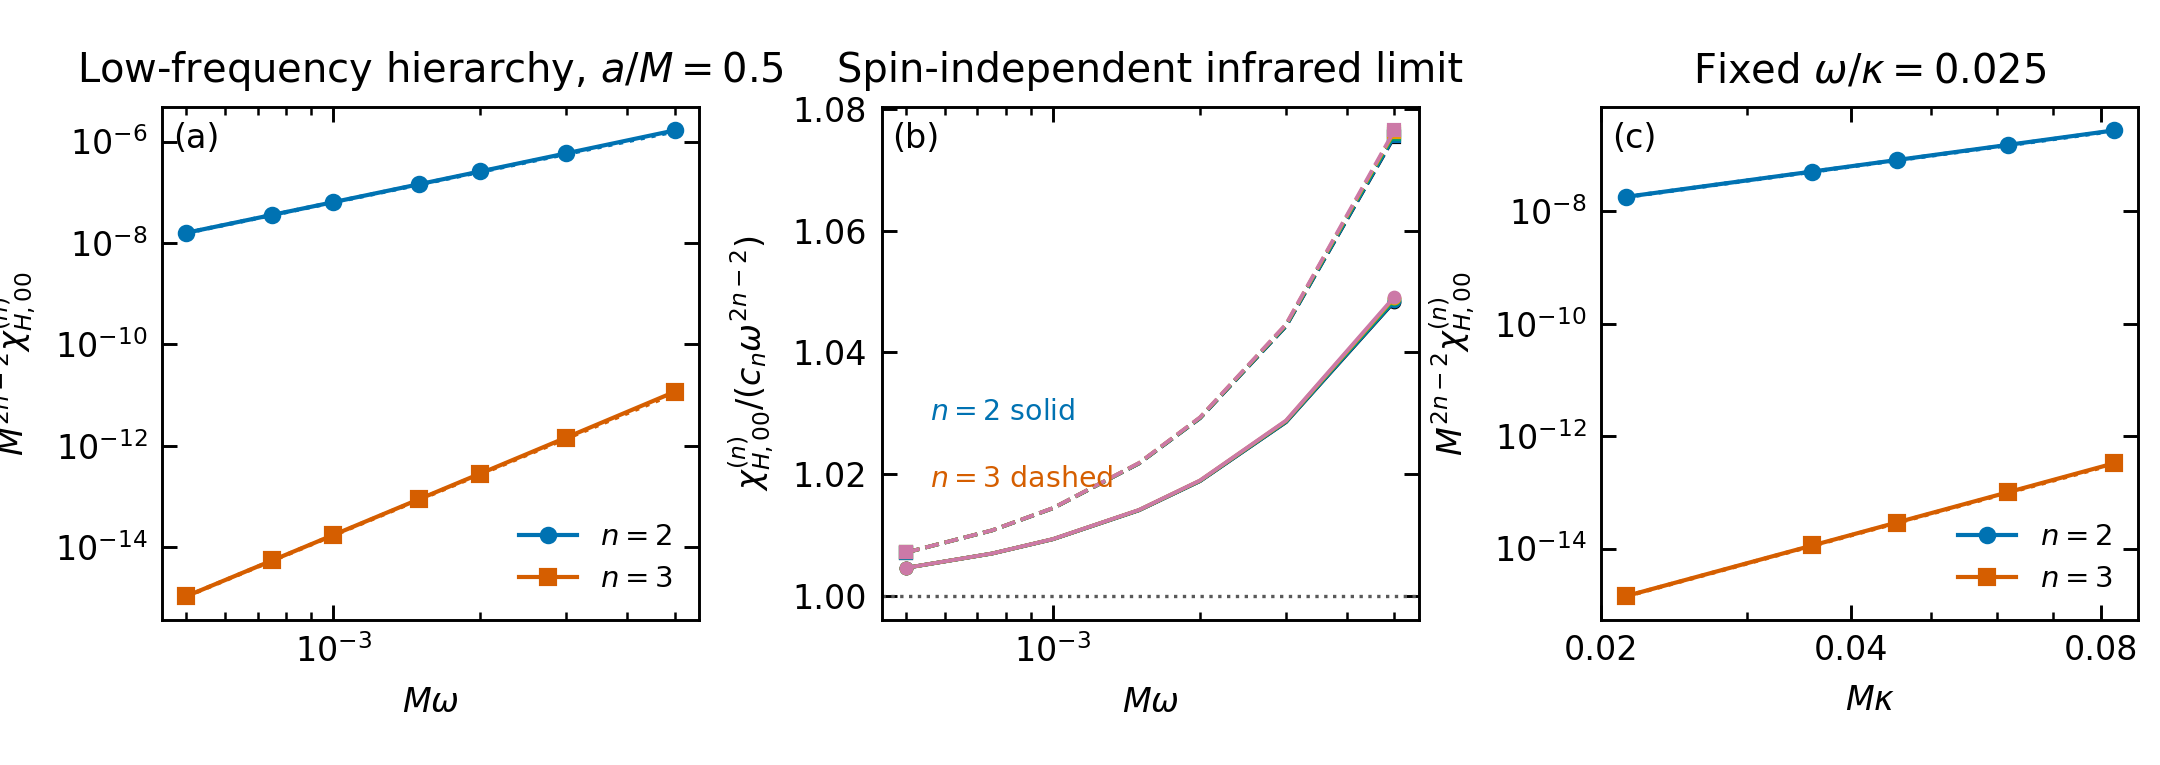
\includegraphics[width=0.98\textwidth]{../../figures/kerr_scalar_power_nonlinearity_l0.png}
\caption{Higher-power scalar-monopole response.  (a) Direct horizon response
for $n=2,3$ at $a/M=0.5$; dotted lines are the analytic leading laws
$c_n\omega^{2n-2}$.  (b) The scaled response divided by $c_n$ for five spins;
solid circles and dashed squares denote $n=2$ and 3.  The near coincidence of
the colored spin curves exhibits the common far-zone limit.  (c) At fixed
$\omega/\kappa=0.025$, the response decreases toward extremality; dotted
curves are $c_n(0.025\kappa)^{2n-2}$.  Points show the $N=q=176$ calculation;
all pass the paired-resolution, linear-balance, and Wronskian tests described
in the text.}
\label{fig:power-l0}
\end{figure*}

\begin{figure*}[t]
\centering
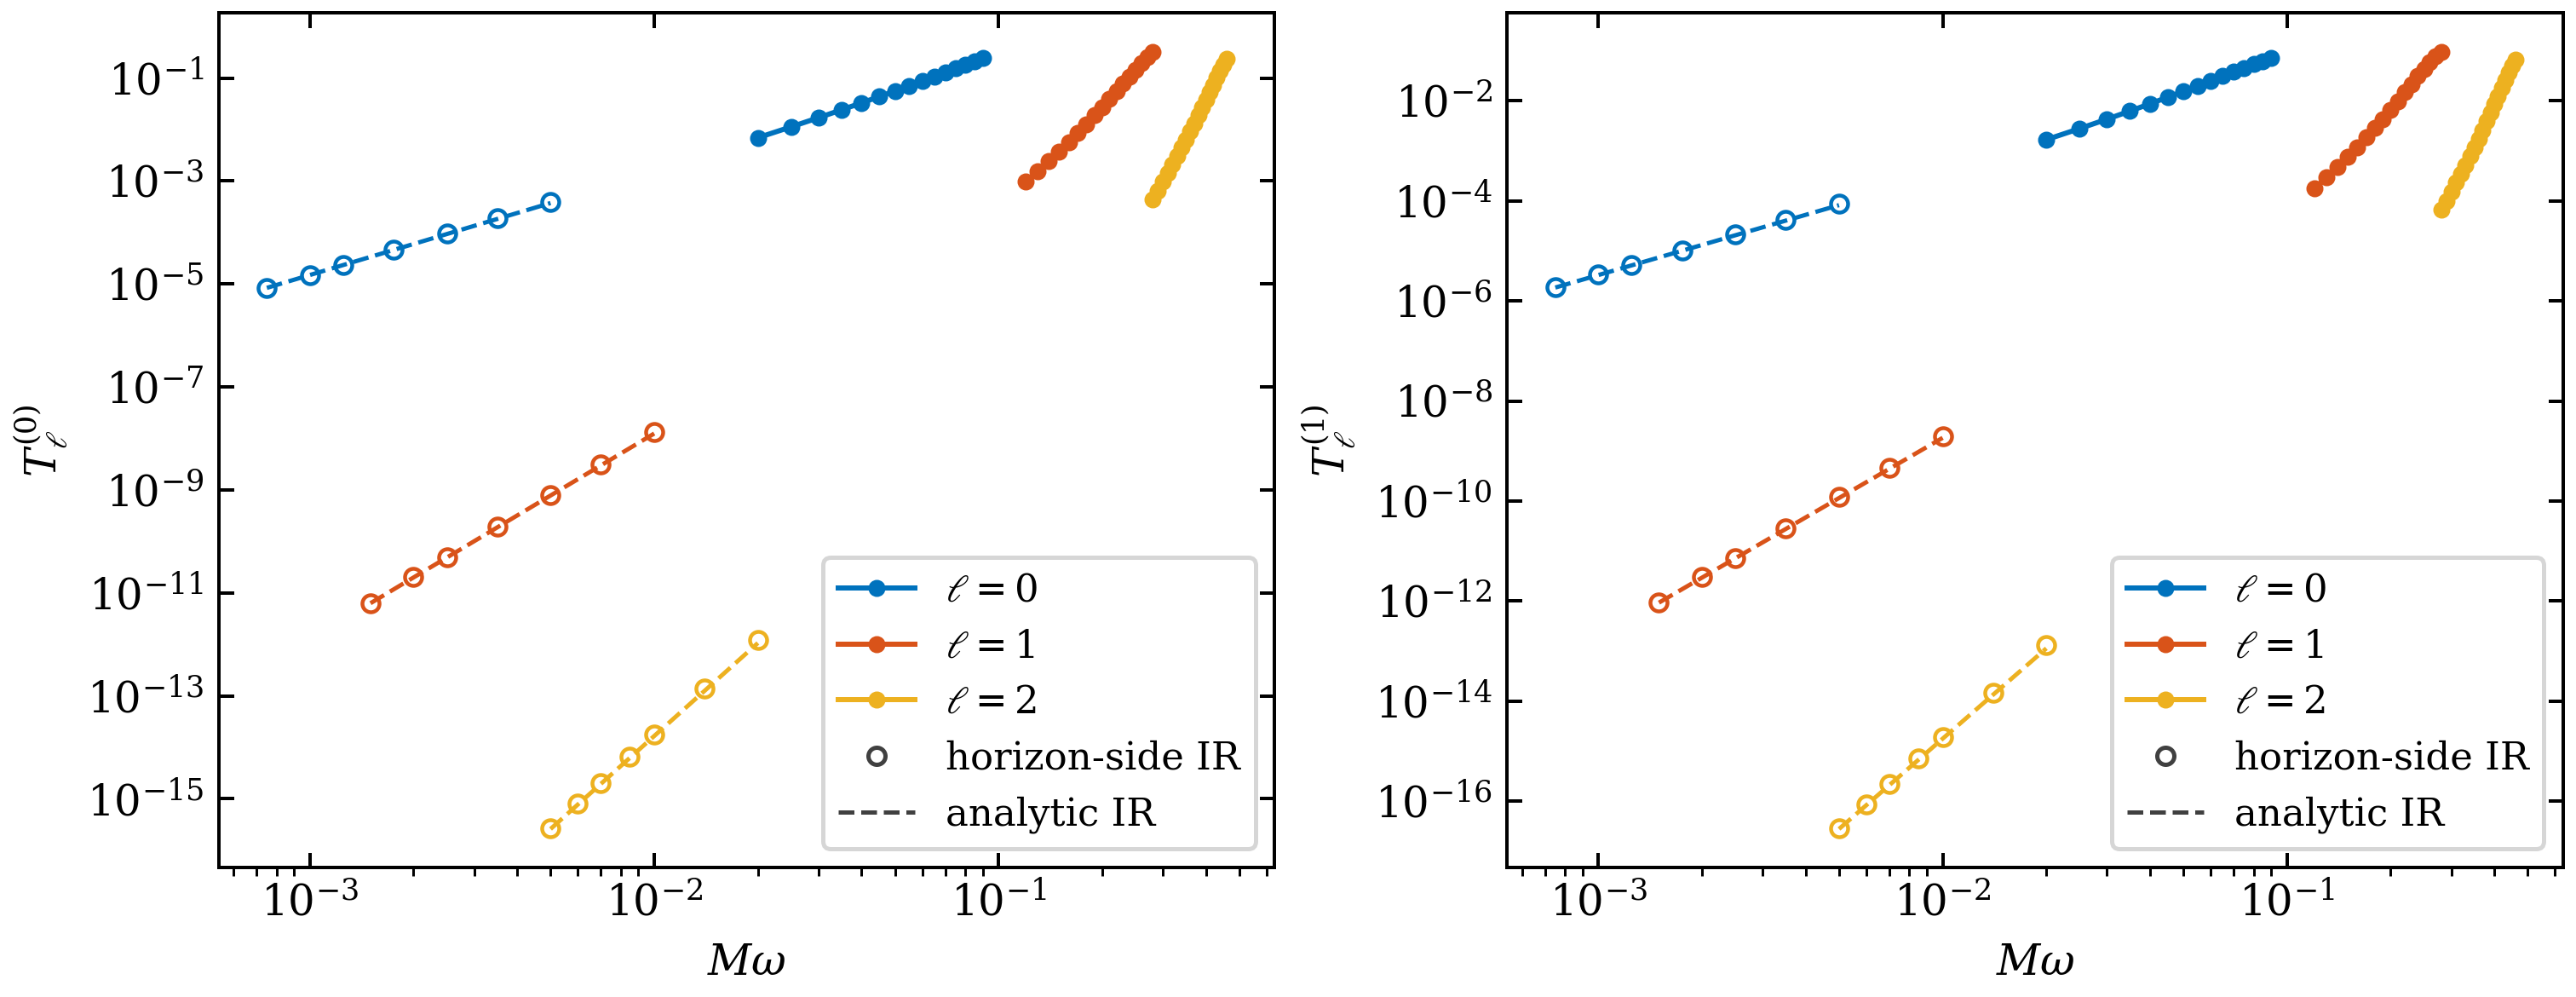
\includegraphics[width=0.92\textwidth]{../../figures/kerr_scalar_low_frequency_axisymmetric.png}
\caption{Low-frequency Kerr diagnostics for $a=0.5$, $m=0$, and
$\ell=0,1,2$.  Left: linear transmission coefficients.  Right:
self-channel nonlinear transmission coefficients.  Filled circles and solid
segments are the dense globally balanced sweep satisfying
$|T^{(1)}+R^{(1)}|\leq10^{-8}$.  Open circles are the higher-resolution
member of the paired horizon-side infrared audit; dashed segments are the
analytic leading laws ${\cal A}^{(i)}_\ell(M\omega)^{2\ell+2}$.  The gap
between the two sets marks loss of reflected-channel cancellation accuracy,
not loss of convergence of the transmitted coefficient.}
\label{fig:lowfreq}
\end{figure*}


\subsection{Near-extremal principal-mode enhancement}
\label{sec:principal20261014}

We next hold the asymptotic incident amplitude and
$y=p/\kappa\ne0$ fixed while approaching extremal rotation, with $m>0$.
The frequency then approaches $\omega_*=m/(2M)$.
This path probes concentration of the incident-normalized field in the Kerr
throat.  We define
\begin{equation}
\sigma=\frac{r_+-r_-}{M},\qquad
\widehat\chi_n=M^{2n-2}\frac{T_n^{(1)}}{T^{(0)}}.
\label{eq:principal-parameters}
\end{equation}
Since $M\kappa=\sigma/[4(1+\sigma/2)]$, the leading powers in $\sigma$
and $M\kappa$ agree.  In the following connection formulas we set $M=1$.
The normalization is unit ingoing horizon amplitude for $R_{\rm in}$ and
unit outgoing infinity amplitude for $R_{\rm up}$.

\subsubsection{The throat equation and its two branches}

Let $X=(r-r_+)/\sigma$.  The exact relations
$\Delta=\sigma^2X(X+1)$ and $(r_+^2+a^2)p=\sigma y/2$ give
\begin{equation}
K=\sigma\left(\frac y2+2r_+\omega X+\sigma\omega X^2\right).
\end{equation}
At fixed $X,y$ the leading radial equation is
\begin{equation}
\frac{d}{dX}\left[X(X+1)\frac{df}{dX}\right]
+\left[\frac{(mX+y/2)^2}{X(X+1)}-\lambda_*\right]f=0,
\label{eq:principal-near-ode}
\end{equation}
where $\lambda_*=A_{\ell m}(m/2)-3m^2/4$ in our angular convention.
In the overlap region the indicial equation gives
\begin{align}
h(h-1)+m^2-\lambda_*&=0,\nonumber\\
h&=\frac12+\sqrt{\frac14+A_{\ell m}(m/2)-\frac{7m^2}{4}}.
\label{eq:principal-weight}
\end{align}
The two branches are $X^{h-1}$ and $X^{-h}$.
The principal class has $h=1/2+i\beta$, $\beta>0$, so both branches have
the same $X^{-1/2}$ amplitude envelope.  The real-weight class has distinct
real exponents.  This classification follows from the radial equation
\cite{BredbergKerrCFT2010}.

The horizon-ingoing solution is
\begin{align}
f_y(X)={}&X^{-iy/2}(1+X)^{i(y/2-m)}\nonumber\\
&\times{}_2F_1(h-im,1-h-im;1-iy;-X).
\label{eq:principal-near-solution}
\end{align}
Continuation to large $X$ yields $f_y\sim c_+X^{h-1}+c_-X^{-h}$, with
\begin{align}
c_+&=\frac{\Gamma(1-iy)\Gamma(2h-1)}
{\Gamma(h-im)\Gamma[h-i(y-m)]},\nonumber\\
c_-&=\frac{\Gamma(1-iy)\Gamma(1-2h)}
{\Gamma(1-h-im)\Gamma[1-h-i(y-m)]}.
\label{eq:principal-near-connection}
\end{align}

\subsubsection{Connection to asymptotically flat radiation}

At extremality set $u=r-1$.  The critical-frequency outer equation becomes
\begin{equation}
u^2R''+2uR'+[m^2(1+u/2)^2-\lambda_*]R=0.
\label{eq:principal-outer-ode}
\end{equation}
Setting $\Psi=uR$ and $z=-imu$ gives the Whittaker equation
\begin{equation}
\frac{d^2\Psi}{dz^2}
+\left[-\frac14+\frac{im}{z}+
\frac{1/4-(h-1/2)^2}{z^2}\right]\Psi=0.
\end{equation}
The solutions normalized to $u^{h-1}$ and $u^{-h}$ are
\begin{align}
R_+(u)&=(-im)^{-h}u^{-1}M_{im,h-1/2}(-imu),\nonumber\\
R_-(u)&=(-im)^{h-1}u^{-1}M_{im,1/2-h}(-imu).
\end{align}
Their incoming amplitudes are
\begin{align}
U_+&=\frac{\Gamma(2h)}{\Gamma(h-im)}(-im)^{-h-im},\nonumber\\
U_-&=\frac{\Gamma(2-2h)}{\Gamma(1-h-im)}(-im)^{h-1-im}.
\label{eq:principal-outer-connection}
\end{align}
These coefficients share a unit-modulus phase determined by the additive
constant in $r_*$.  We use the principal branch of $\log(-im)$ consistently.
The near hypergeometric and outer Whittaker representations implement the
leading near-extremal analytic connection.  MST supplies the full-frequency
series and connection structure\cite{MST1996}; its renormalized angular
momentum $\nu$ and the throat index $h$ label the respective representations.

In the overlap region $u\simeq\sigma X$, matching gives
\begin{align}
B^{\rm inc}&\sim c_+U_+\sigma^{1-h}+c_-U_-\sigma^h\nonumber\\
&=\sigma^{1/2}{\cal D}(\theta),\qquad\theta=\beta\ln\sigma,\nonumber\\
{\cal D}(\theta)&=c_+U_+e^{-i\theta}+c_-U_-e^{i\theta}.
\label{eq:principal-incidence}
\end{align}
Thus fixed-incident normalization yields
\begin{equation}
|R_H^{(0)}|^2\sim\frac{\sigma^{-1}}{|{\cal D}(\theta)|^2}.
\label{eq:principal-density}
\end{equation}
The near-critical horizon flux carries an additional factor $p\propto\sigma$.
Consequently the linear absorption is finite and log-phase dependent, with
$T^{(0)}\sim y/[m|{\cal D}|^2]$ in $M=1$ units.

\subsubsection{The nonlinear source integral and the envelope law}

Choose near solutions $\psi_+\sim X^{h-1}$ and $\psi_-\sim X^{-h}$.
The outgoing Whittaker solution $u^{-1}W_{im,h-1/2}(-imu)$ has overlap
coefficients
\begin{align}
g_+&=\frac{\Gamma(1-2h)}{\Gamma(1-h-im)}(-im)^h,\nonumber\\
g_-&=\frac{\Gamma(2h-1)}{\Gamma(h-im)}(-im)^{1-h}.
\end{align}
Its near-zone form is $R_{\rm up}\sim\sigma^{-1/2}\gamma_\theta$, where
\begin{equation}
\gamma_\theta=g_+e^{i\theta}\psi_++g_-e^{-i\theta}\psi_-.
\end{equation}
The constant near Wronskian and its physical counterpart are
\begin{align}
w_\theta&=X(X+1)(f_y\gamma_\theta'-\gamma_\theta f_y'),\nonumber\\
W&\sim\sigma^{1/2}w_\theta.
\end{align}
The covariant source weight at the limiting horizon is
$C_H^{(n)}=C^{(0,n)}_{\ell\ell m}+C^{(2,n)}_{\ell\ell m}$.
Since $dr=\sigma\,dX$, the Green projection gives the finite leading
unit-horizon coefficient
\begin{equation}
{\cal A}_n(\theta)=-\frac{C_H^{(n)}}{w_\theta}
\int_0^\infty\gamma_\theta|f_y|^{2n}f_y\,dX.
\label{eq:principal-source-integral}
\end{equation}
At $X=0$ the amplitude envelope is bounded.  At large $X$ the integrand
envelope is $X^{-n-1}$, so the integral converges for every positive integer
$n$.  The factors $\sigma^{-1/2}$ from $R_{\rm up}$, $\sigma$ from $dr$,
and $\sigma^{-1/2}$ from $1/W$ cancel.  The remaining real power in the
fixed-incident response therefore comes from $|B^{\rm inc}|^{-2n}$:
\begin{align}
\widehat\chi_n&=\sigma^{-n}{\cal F}_n(y,\theta)+o(\sigma^{-n}),\nonumber\\
{\cal F}_n(y,\theta)&=\frac{2\operatorname{Re}{\cal A}_n(\theta)}
{|{\cal D}(\theta)|^{2n}}.
\label{eq:principal-law}
\end{align}
The expansion applies on compact parameter sets where the matching
denominators stay bounded away from zero.  At a zero of
$\operatorname{Re}{\cal A}_n$, the next term controls the flux response.
Transforming $\theta\mapsto\theta+\pi$ changes the signs of $\gamma,w$ and
$\mathcal D$ while preserving $\mathcal A_n$ and $|\mathcal D|$.
The leading coefficient hence has logarithmic period $\pi/\beta$.
The envelope power is $-n$, and the two-branch interference determines its
log-periodic modulation.

For reproducible coefficient evaluation, write $\gamma=a_\theta f_y+
b_\theta f_y^*$.  The horizon current gives
$|c_+|^2-|c_-|^2=-y/(2\beta)$ and $w_\theta=iyb_\theta$.
Let $G_+=g_+e^{i\theta}$, $G_-=g_-e^{-i\theta}$ and
$d_c=|c_+|^2-|c_-|^2$.  Then
\begin{align}
a_\theta&=(G_+c_+^*-G_-c_-^*)/d_c,\nonumber\\
b_\theta&=(-G_+c_-+G_-c_+)/d_c,\nonumber\\
{\cal A}_n&=\frac{iC_H^{(n)}}{y}
\left(\frac{a_\theta}{b_\theta}I_n^{\rm osc}+I_n^{\rm abs}\right),\nonumber\\
I_n^{\rm osc}&=\int_0^\infty f_y^2|f_y|^{2n}\,dX,\qquad
I_n^{\rm abs}=\int_0^\infty|f_y|^{2n+2}\,dX.
\label{eq:principal-integral-evaluation}
\end{align}
Equations~\eqref{eq:principal-near-connection}--\eqref{eq:principal-integral-evaluation}
specify the leading prediction with zero fitted parameters.

\subsubsection{Real weights and the perturbative domain}

For a real nondegenerate $h>1/2$, the dominant incident connection has
$B^{\rm inc}\sim c_+U_+\sigma^{1-h}$ and the incident-normalized near
field scales as $\sigma^{h-1}$.  The projected Green integrand in the
overlap region scales as $X^{2n(h-1)-1}$.
For $1/2<h<1$ the upper integral converges and the throat contribution
has power $\sigma^{2n(h-1)}$.  For $h>1$, the matching upper limit
$X\sim\sigma^{-1}$ supplies $\sigma^{-2n(h-1)}$; the resulting
order-unity contribution is determined by the full outer matching.
At $h=1$ the upper integral has logarithmic behavior.
This convergence criterion specifies when a local throat power controls
the complete observable.  The real-weight channel $(1,1)$ has
$h=1.1706059743$ and belongs to the upper-limit-sensitive class.

Define $g_n=\epsilon_n/M^{2n-2}$ and the dimensionless complex horizon
response $\widehat\rho_n$, with
$\widehat\chi_n=2\operatorname{Re}\widehat\rho_n$.
The leading field correction has
$\widehat\rho_n\sim\sigma^{-n}{\cal A}_n/|{\cal D}|^{2n}$.
The relative horizon-field and flux corrections obey, respectively,
\begin{equation}
\begin{split}
|g_n|\,|{\cal A}_{\rm in}|^{2n}|\widehat\rho_n|&\ll1,\\
|g_n|\,|{\cal A}_{\rm in}|^{2n}|\widehat\chi_n|&\ll1.
\end{split}
\label{eq:principal-validity}
\end{equation}
The field condition controls both the horizon amplitude and its phase.
On principal-mode intervals with a bounded nonzero typical coefficient,
the expansion parameter scales as
$|g_n||{\cal A}_{\rm in}|^{2n}(M\kappa)^{-n}$.
This identifies the shrinking weak-coupling domain near extremality.

\subsubsection{Expanded numerical verification}

\begin{table}[t]
\caption{Critical scalar angular eigenvalues and principal weights at
$a/M=1$, $M\omega=m/2$, with $h=1/2+i\beta$.}
\label{tab:principal-weights20261014}
\begin{ruledtabular}\begin{tabular}{ccc}
$(\ell,m)$ & $A_{\ell m}$ & $\beta$\\
$(2,2)$ & 5.8551625746 & 0.9459584692 \\
$(3,3)$ & 11.7447939547 & 1.9378354020 \\
$(4,4)$ & 19.6267345276 & 2.8501342902 \\
\end{tabular}\end{ruledtabular}\end{table}
\begin{table*}[t]
\caption{Parameter-free leading matching at $a/M=0.999999$.
Relative matching differences are in percent. $\delta_{\rm pair}$ is the
maximum change across all spins and orders under $(N,q)=(384,32)\to(448,48)$
with log-horizon quadrature. $\delta_{\rm old}$ compares the refined response
with the previous global $q=3072$ rule. Independent panel-order,
lower-limit and matching-radius checks are described in the text.}
\label{tab:principal-verification20261014}
\begin{ruledtabular}\begin{tabular}{ccccccc}
$(\ell,m)$ & $y$ & $n=1$ (\%) & $n=2$ (\%) & $n=3$ (\%) & $\delta_{\rm pair}$ & $\delta_{\rm old}$\\
$(2,2)$ & -0.5 & 1.925 & 2.403 & 2.422 & $4.13\times10^{-9}$ & $6.49\times10^{-8}$\\
$(2,2)$ & 0.5 & 0.825 & 0.964 & 0.894 & $8.43\times10^{-11}$ & $1.39\times10^{-6}$\\
$(2,2)$ & 1 & 0.782 & 0.717 & 0.581 & $1.26\times10^{-11}$ & $4.15\times10^{-6}$\\
$(3,3)$ & -0.5 & 0.202 & 0.516 & 0.834 & $6.55\times10^{-9}$ & $6.16\times10^{-8}$\\
$(3,3)$ & 0.5 & 0.111 & 0.307 & 0.506 & $1.26\times10^{-10}$ & $1.09\times10^{-6}$\\
$(3,3)$ & 1 & 0.054 & 0.179 & 0.305 & $1.41\times10^{-11}$ & $1.26\times10^{-5}$\\
$(4,4)$ & -0.5 & 0.042 & 0.343 & 0.665 & $1.65\times10^{-9}$ & $1.17\times10^{-7}$\\
$(4,4)$ & 0.5 & 0.066 & 0.294 & 0.537 & $9.19\times10^{-10}$ & $7.49\times10^{-7}$\\
$(4,4)$ & 1 & 0.028 & 0.183 & 0.380 & $9.10\times10^{-11}$ & $2.27\times10^{-5}$\\
\end{tabular}\end{ruledtabular}\end{table*}
The refined $81$-point grid has a maximum paired real-response change of
$6.55\times10^{-9}$ and a complex-response change of $3.25\times10^{-9}$.
Six representative cases also vary the panel order and lower integration
limit at fixed $N=448$, giving a maximum response change of
$3.91\times10^{-13}$, and vary $r_{\rm match}/M=8,12,16$, giving a
maximum response range of $5.42\times10^{-9}$.
The homogeneous fields are unchanged by the quadrature refinement;
their maximum off-grid radial relative residual is $1.37\times10^{-8}$
and their maximum coefficient tail is $6.82\times10^{-14}$.
The maximum normalized interference-balance error is $2.47\times10^{-9}$.
The original absolute flux gate is met by $60$ points and is recorded
separately from the local and paired-response criteria.
The maximum absolute interference-balance error is $3.32\times10^{-6}$. The two analytic integral settings differ by at most $1.96\times10^{-12}$ in the recorded relative integral diagnostic. The analytic log-period test has a maximum relative difference of $4.38\times10^{-13}$.


We evaluate the full covariant source for $(\ell,m)=(2,2),(3,3),(4,4)$,
$n=1,2,3$, $y=-0.5,0.5,1$, and
$a/M=0.9999,0.99999,0.999999$.
The grid has $81$ physical parameter points.  Refined production uses
$N=448$ and $48$ Gauss nodes per logarithmic panel, with
$r_{\rm match}=12M$.  A paired $N=384$, $32$-node calculation supplies
an additional $162$ solver calls across the grid; the previous $324$
global-rule calls remain archived for comparison.
For the inner Green integral we use $t=\ln[(r-r_+)/(r_+-r_-)]$,
with panel lengths at most unity.  The interval below
$\delta=(r_+-r_-)e^{t_{\min}}$ is integrated using the leading horizon
power.  For example, with the same tortoise convention,
\begin{equation}
\int_0^\delta e^{-2ipr_*(r_++s)}\,ds
=\frac{\delta e^{-2ipr_*(r_++\delta)}}{1-iy}
+\mathcal O\!\left(\frac{\delta^2}{r_+-r_-}\right).
\label{eq:log-horizon-endpoint-integral}
\end{equation}
The regular prefactors are evaluated at the horizon in this short interval.
The refined grid uses $t_{\min}=-34$; the representative checks vary
$t_{\min}=-26,-30,-34$ and panel orders $32,48,64$.
This procedure preserves the exact horizon in both the spectral equation
and the Green integral.  Stable evaluation in the positive distance $s$
avoids subtracting nearly equal radii in the tortoise logarithms.
The near integrals use $t=\ln X$ with two independent settings:
$t\in[-30,30]$, $12$ Gauss nodes per unit interval, and
$t\in[-36,36]$, $20$ nodes per interval.  Special functions are evaluated
with $32$ decimal digits and accumulated quadratures use double precision.
Angular eigenvalues and source projections use the critical spheroidal
functions.  This procedure fixes all prediction coefficients from the
field equation and normalization.

\begin{figure*}[t]
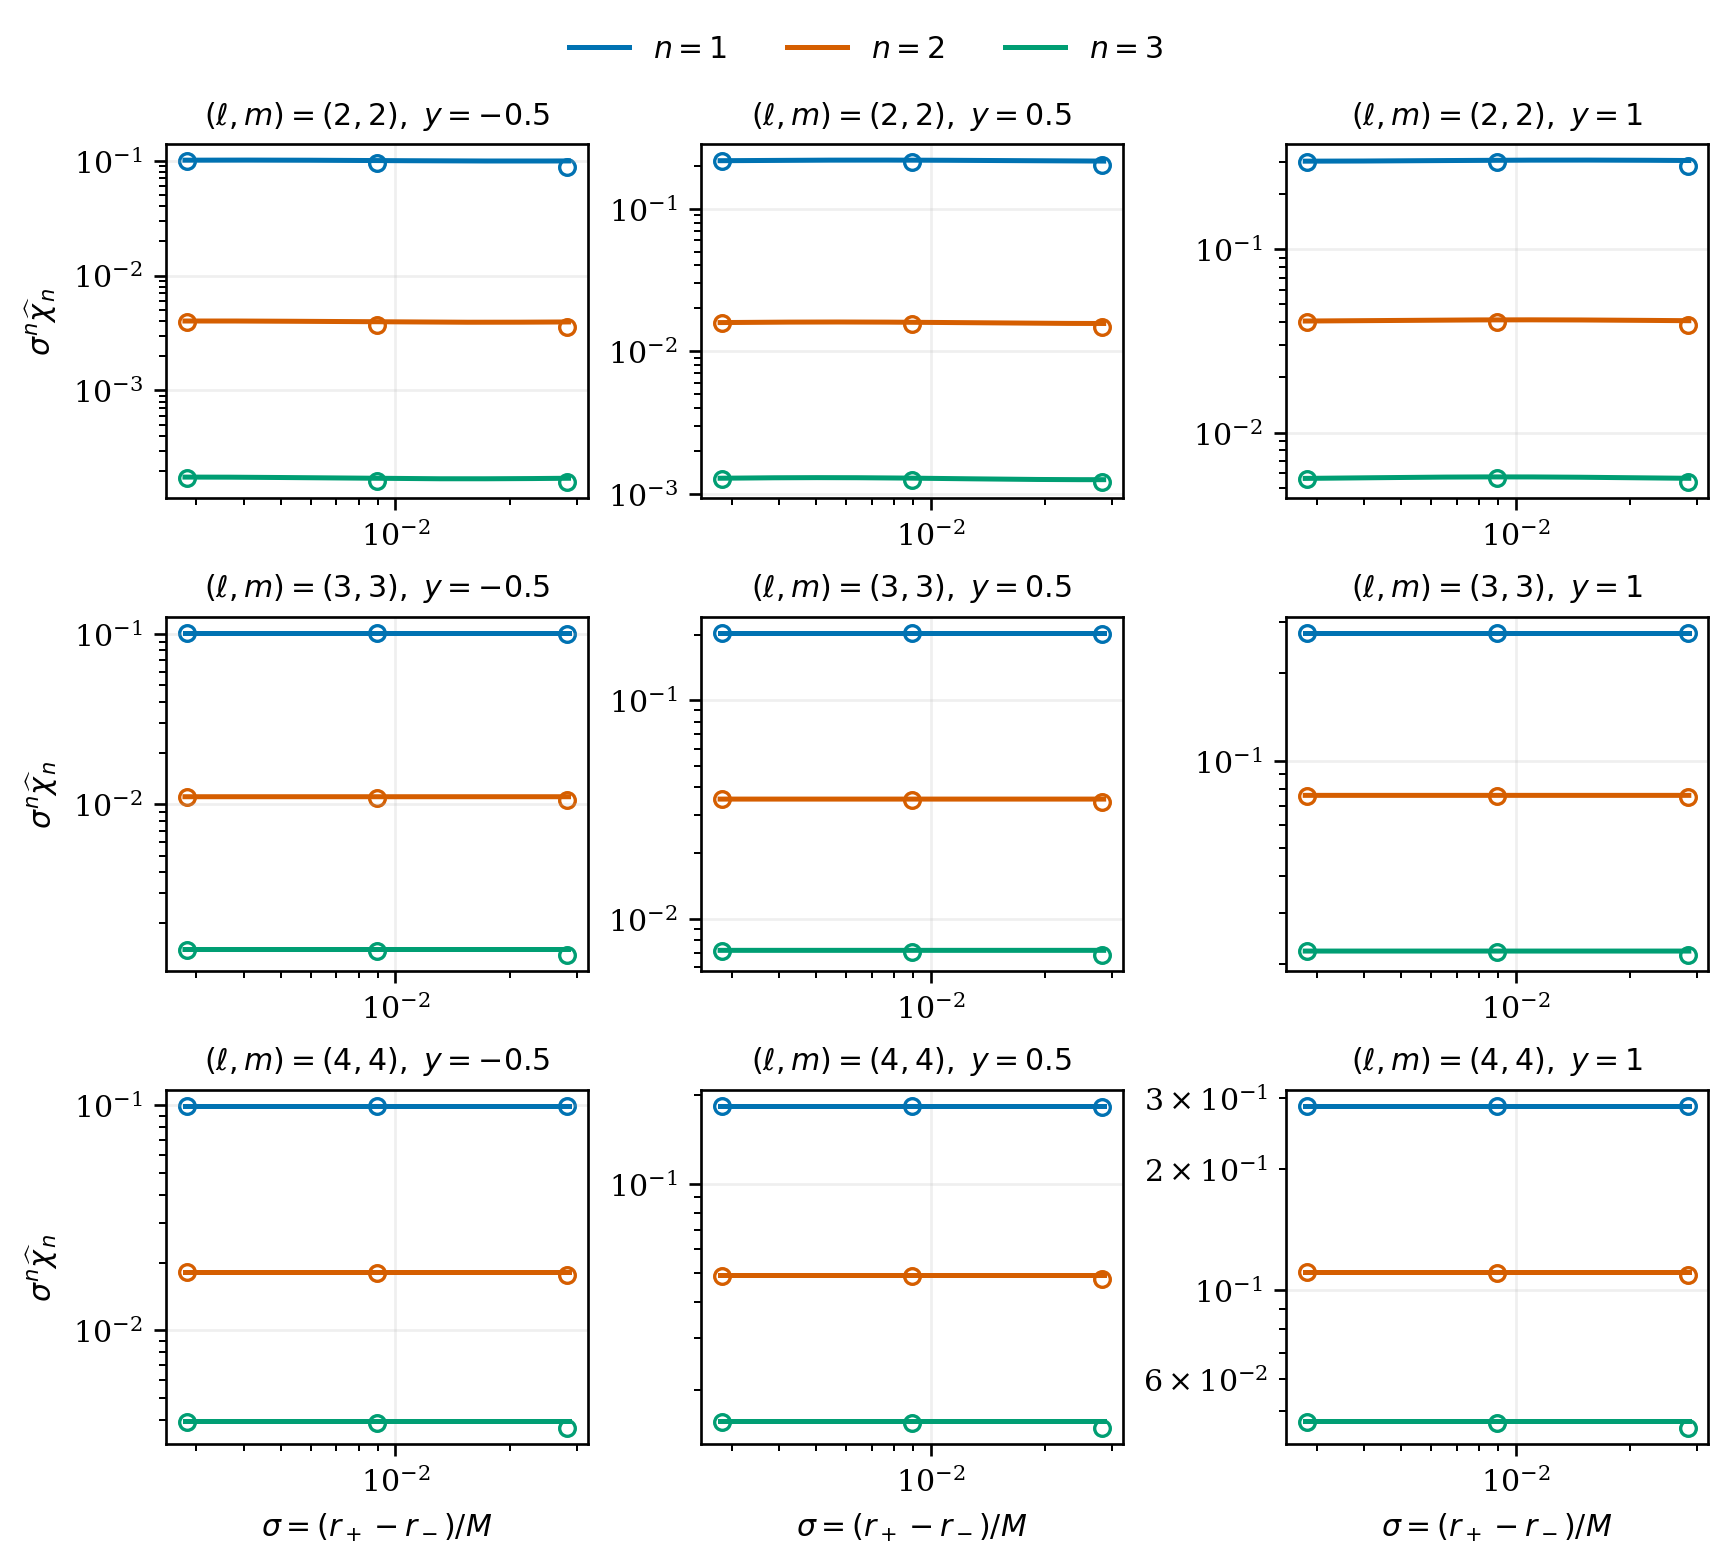
\includegraphics[width=0.96\textwidth]{../../figures/kerr_scalar_principal_log_refined_20261014.png}
\caption{Principal-mode response coefficients after removing the predicted
envelope, $\sigma^n\widehat\chi_n$.  Rows are $(2,2),(3,3),(4,4)$ and
columns are $y=-0.5,0.5,1$.  Colors label $n=1,2,3$.  Lines are the
parameter-free analytic functions evaluated at $180$ display locations;
symbols are the independently computed full Kerr spectral points.
Each numerical series has three spins and paired spectral/logarithmic-panel
resolutions.  The solid functions retain the two-branch logarithmic phase.
The comparison tests the leading coefficient as well as the envelope power.}
\label{fig:principal-expanded}
\end{figure*}

The acceptance criteria for this large-response experiment combine
paired changes of the real and complex horizon response, spectral tails,
field-dependent off-grid radial residuals and separately recorded flux
interference errors.  Both absolute $|T_n^{(1)}+R_n^{(1)}|$ and relative
$|T_n^{(1)}+R_n^{(1)}|/(|T_n^{(1)}|+|R_n^{(1)}|)$ are retained.
The axisymmetric figures continue to use their original absolute gate.
The principal-response figure uses the local and paired-response criteria
reported with Table~\ref{tab:principal-verification20261014}; the CSV also
identifies which points pass the original absolute gate.
The thresholds are $10^{-5}$ for both paired horizon-response changes,
$10^{-4}$ for the independent quadrature change, $10^{-6}$ for the
off-grid radial residual, $10^{-8}$ for the spectral tail, and $10^{-6}$
for the normalized interference balance.  The original absolute gate is
$10^{-8}$.  These tolerances are applied uniformly across the grid.
The physical flux correction multiplies each coefficient and its absolute
numerical error by $\epsilon_n|{\cal A}_{\rm in}|^{2n}$.

The observed resolution changes quantify numerical error, while the
difference from the parameter-free prediction quantifies the finite-$\sigma$
correction to the leading matched approximation.
The envelope in Eq.~\eqref{eq:principal-law} follows analytically from
the equal real parts of the two principal branches and the convergence of
the nonlinear source integral.  Three-spin slope estimates provide a
finite-window diagnostic; the coefficient comparison supplies the direct
test of the derived response function.

\subsubsection{Flux-response zeros and an enhanced phase response}
\label{sec:phase-flux-separation}

The complex coefficient provides an additional observable distinction.
Define $\psi_n=\operatorname{Im}\widehat\rho_n$;
its first-order transmitted phase shift is
$g_n|\mathcal A_{\rm in}|^{2n}\psi_n$.
Generalizing Eq.~\eqref{eq:kerr-tail-decomposition} to the self channel of
$|\Phi|^{2n}\Phi$, replace $P$ by $P_n=r^2C^{(0,n)}+a^2C^{(2,n)}$
and $|R^{\rm in}|^2$ by $|R^{\rm in}|^{2n}$ in $J_{\rm d},J_{\rm o}$.
Writing $q_{\mathrm r}=B^{\rm ref}/B^{\rm inc}$ gives
\begin{align}
\widehat\chi_n&=-\frac{M^{2n-2}\operatorname{Im}(q_{\mathrm r}J_{{\rm o},n})}
{\omega|B^{\rm inc}|^{2n}},\nonumber\\
\psi_n&=\frac{M^{2n-2}[J_{{\rm d},n}+
\operatorname{Re}(q_{\mathrm r}J_{{\rm o},n})]}
{2\omega|B^{\rm inc}|^{2n}}.
\label{eq:phase-flux-projections}
\end{align}
Thus a zero of the imaginary interference projection makes the
first-order energy-flux correction vanish while the real projection
can retain a phase response.  For principal modes both components carry
the $\sigma^{-n}$ envelope, with distinct phase-dependent coefficients.

We compute $27$ further points for $(\ell,m)=(2,2)$, $n=1,2,3$,
$y=1,2,4$, and the same three spins, each at paired resolutions.
The maximum relative changes are $2.36\times10^{-11}$ for the phase
and $5.28\times10^{-8}$ for the flux response.
At $a/M=0.999999$, $n=3$, $y=2$, we find
$\psi_3=2.4132\times10^4$ and $\widehat\chi_3=363.07$;
at $y=4$ they are $1571.09$ and $-0.0102804$, respectively.
These samples establish phase-dominated response coefficients within the
tested detuning range.

A resolved zero occurs near $y_\star=2.41954$ for this $n=3$ channel.
Independent calculations at $N=448,576$, panel orders $48,64$, and
$r_{\rm match}/M=8,12,16$ preserve the opposite signs at
$y_\star\pm2\times10^{-4}$.
At the common central estimate they give
$|\widehat\chi_3|\le5.73\times10^{-9}$ and
$\psi_3\simeq1.0316\times10^4$.
The sign bracket, rather than a relative error at zero, establishes the
crossing.  The first-order balance then gives $R_3^{(1)}=-T_3^{(1)}$,
so both energy-flux derivatives vanish at the limiting zero.
The phase coefficient retains its finite value there.

\begin{figure*}[t]
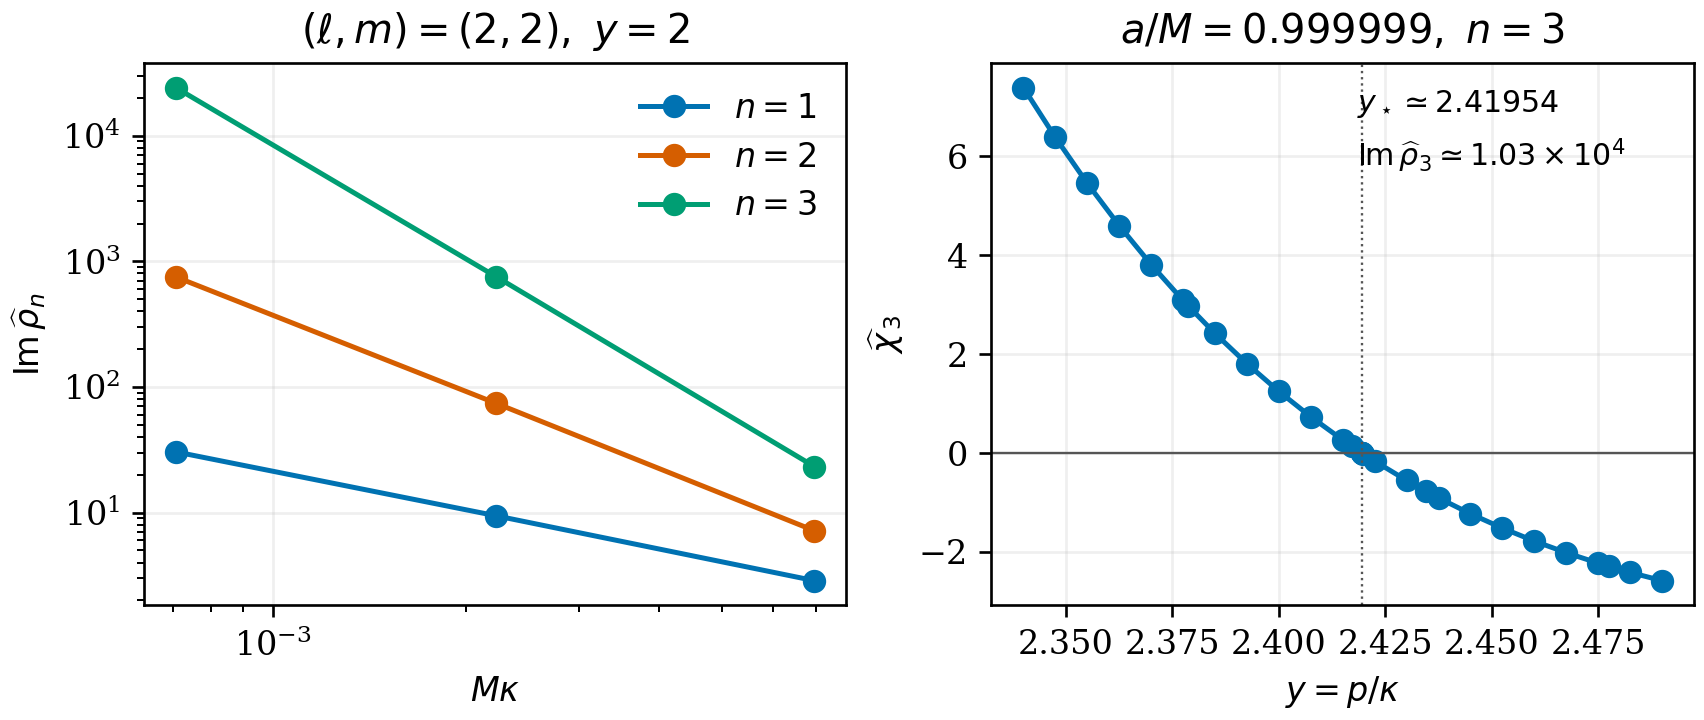
\includegraphics[width=0.96\textwidth]{../../figures/kerr_scalar_phase_flux_separation_20261014.png}
\caption{Phase and flux components of the nonlinear response.
Left: transmitted phase coefficients for $(2,2)$ at fixed $y=2$ and
$n=1,2,3$ across three spins.  Right: the $n=3$ flux-response crossing
at $a/M=0.999999$; circles include $21$ uniformly spaced direct evaluations
on $2.34\le y\le2.49$ and the root-search samples.
Joining segments are visual guides.  The phase coefficient at the
crossing is about $1.03\times10^4$.  Separate degree, panel-order and
matching-radius checks bracket the zero as described in the text.}
\label{fig:phase-flux-separation}
\end{figure*}

We independently reconstruct the sourced field on $1\le X\le8$ at this
detuning and differentiate its Chebyshev interpolant.  At reconstruction
degrees $16,24,32,48,64$, the maximum field-dependent relative residuals
are $0.128$, $9.23\times10^{-4}$, $4.77\times10^{-6}$,
$9.10\times10^{-9}$, and $6.62\times10^{-8}$, respectively.
The coefficient tail falls from $3.84\times10^{-3}$ to
$4.33\times10^{-15}$; the full degree sequence displays the
high-degree differentiation floor.  This local test includes the source
term in the residual denominator and supplements the global integral
and sign-bracket checks.
The horizon perturbative condition at a flux zero continues to involve
$|g_n||\mathcal A_{\rm in}|^{2n}|\widehat\rho_n|$.
Finite-coupling energy-flux changes require the second-order field as
well as the square of the first-order field.

\subsection{Kerr-to-Schwarzschild continuity}

As a limiting-case check independent of external reference calculations, we
hold $(\ell,m,M\omega)=(2,0,0.52)$ fixed and sweep the dimensionless spin from
$a/M=0$ to $0.5$.  The scalar spheroidal eigenvalue, the covariant source
projection, the scattering amplitudes, and both flux coefficients are
recomputed at every spin.  At $a=0$ the angular basis becomes spherical and the
endpoint formulation reduces to the Schwarzschild spectral route; no radial
endpoint is removed or replaced by a finite horizon cutoff.  Figure~\ref{fig:spin-limit}
shows that $T^{(1)}$ and $-R^{(1)}$ vary smoothly from the $a=0$ value, while
Table~\ref{tab:spin-limit} records the balance and Wronskian diagnostics for
the same points.  The largest absolute first-order balance residual in this
scan is $1.4\times10^{-12}$ and the largest linear balance residual is below
$1.2\times10^{-11}$.  This experiment is a continuity and implementation
check; it is not used as an external reference result or as a claim that the Kerr and
Schwarzschild coefficient conventions are identical without the conversion in
Appendix~\ref{app:flux}.

\begin{figure*}[t]
\centering
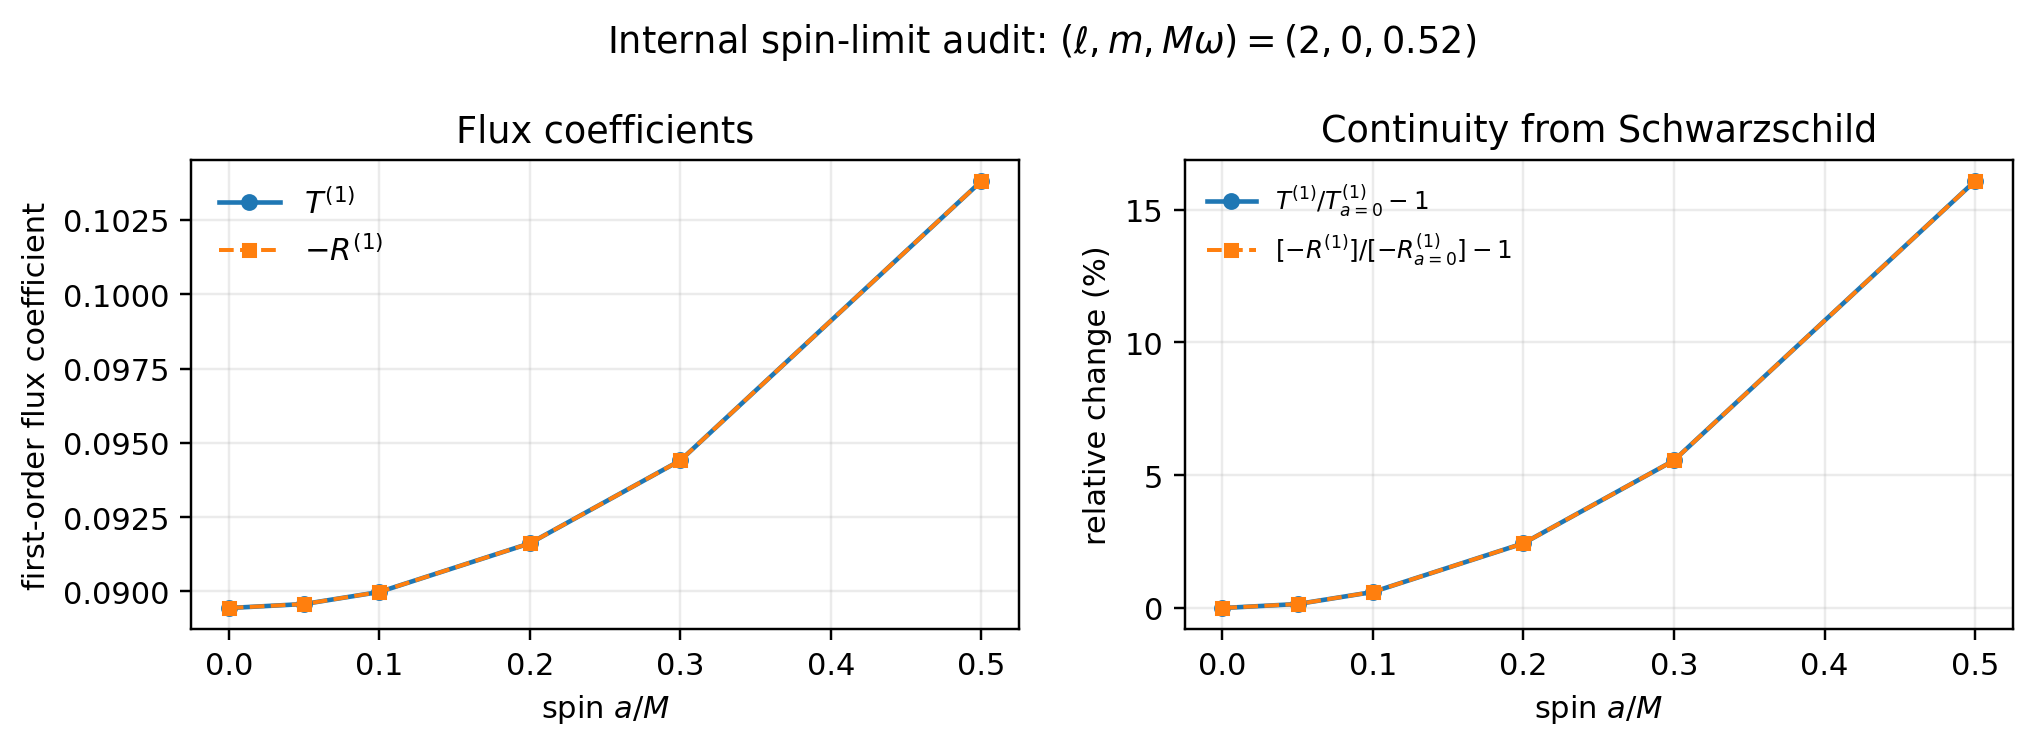
\includegraphics[width=0.92\textwidth]{../../figures/kerr_scalar_spin_limit.png}
\caption{Internal Kerr-to-Schwarzschild continuity test at fixed
$(\ell,m,M\omega)=(2,0,0.52)$.  The first-order transmission coefficient and
$-R^{(1)}$ remain paired by the flux balance while changing smoothly with
$a/M$.  The right panel normalizes both coefficients to the $a=0$ value; all
points use the endpoint-inclusive spectral solver and are accepted by the
first-order balance check.}
\label{fig:spin-limit}
\end{figure*}

\begin{table*}[t]
\caption{Internal Kerr-to-Schwarzschild spin-limit audit for
$(\ell,m,M\omega)=(2,0,0.52)$.  The entries use the same fixed-incident
normalization as the production coefficients.  The two balance columns are
$T^{(0)}+R^{(0)}-1$ and $T^{(1)}+R^{(1)}$, respectively.}
\label{tab:spin-limit}
\begin{ruledtabular}
\begin{tabular}{c c c c c c}
$a/M$ & $T^{(1)}$ & $R^{(1)}$ & $|\delta_0|$ & $|\delta_1|$ & $|\delta_W|$\\
\hline
0.00 & $8.94395\times10^{-2}$ & $-8.94395\times10^{-2}$ & $1.1\times10^{-12}$ & $3.8\times10^{-13}$ & $2.6\times10^{-16}$\\
0.05 & $8.95742\times10^{-2}$ & $-8.95742\times10^{-2}$ & $9.8\times10^{-12}$ & $1.1\times10^{-12}$ & $3.3\times10^{-16}$\\
0.10 & $8.99794\times10^{-2}$ & $-8.99794\times10^{-2}$ & $3.7\times10^{-12}$ & $4.9\times10^{-13}$ & $0$\\
0.20 & $9.16178\times10^{-2}$ & $-9.16178\times10^{-2}$ & $4.3\times10^{-13}$ & $7.6\times10^{-14}$ & $1.8\times10^{-16}$\\
0.30 & $9.44095\times10^{-2}$ & $-9.44095\times10^{-2}$ & $1.1\times10^{-11}$ & $1.3\times10^{-12}$ & $1.8\times10^{-16}$\\
0.50 & $1.03814\times10^{-1}$ & $-1.03814\times10^{-1}$ & $6.0\times10^{-12}$ & $1.2\times10^{-12}$ & $0$\\
\end{tabular}
\end{ruledtabular}
\end{table*}

\section{Discussion and conclusions}

The complex fixed-incident response connects the frequency profile of
nonlinear Kerr scattering to the wave amplitude available to drive the
local interaction.  Resonance peaks and post-resonance decay describe its
finite-frequency structure.  The fixed-spin infrared limit determines how
the source scales after the penetration factor cancels in the fractional
response.  The fixed-$p/\kappa$ near-extremal limit determines how throat
concentration enhances that response.  The Green-function projection and
its flux--phase decomposition provide the common framework for these
three regimes.  This organization follows the Schwarzschild scattering
construction while retaining the Kerr horizon frequency, spheroidal
functions, and covariant source.  All coefficients use the same
fixed-incident normalization.

The cubic axisymmetric sweep at $a/M=0.5$ resolves peak centers at
$M\omega_p=0.1306,0.3101,0.5026$ for $\ell=0,1,2$.
The centers vary by at most $6.7\times10^{-4}$ under the stated fit-window
changes and lie above the corresponding fundamental scalar QNM real
parts by $16.2\%,4.1\%,2.2\%$.
The nonlinear source projection and its phase enter the same Green
coefficient as the homogeneous scattering kernel.  The resulting
source-weighted resonance provides a real-frequency nonlinear observable
on the QNM scale.  The fitted widths describe the measured profile;
extracting modal residues requires a complex-frequency Green-function
projection.

The post-resonance tails favor an exponential over a power law, with
$\Delta\mathrm{AICc}=97.9,48.2,23.8$ in the resolved windows.
The exact decomposition in Eq.~\eqref{eq:kerr-tail-decomposition} attributes
the first-order flux correction to the linear reflected amplitude times
an oscillatory nonlinear source projection.  It also separates a direct
phase-shift contribution.  The Schwarzschild-inspired
$(M\omega)^{-1/2}$ prefactor improves the tail residuals for $\ell=1,2$
and changes the fitted decay scales in all three channels.
For $\ell=0$, its fitted temperature is within $1.3\%$ of the Kerr $T_H$;
for $\ell=1,2$, a free scale captures the residual modal dependence.
The numerical conclusion is exponential suppression in the stated
post-resonance windows, with a quantitatively tested dependence on the
algebraic prefactor.  A Kerr asymptotic exponent requires the corresponding
complex-radial analysis of the reflection amplitude and source integral.

At fixed subextremal spin, the infrared response has an interaction-order
hierarchy.  At fixed nonzero $p/\kappa$, principal-mode scattering near
extremality has an inverse-surface-gravity envelope with logarithmic
modulation.  The matched source integrals and asymptotically flat incident
normalization determine both limits.

The flux formulation separates three quantities that can otherwise be
confused: a unit-horizon Green coefficient, the relative fixed-incident field
response, and the physical correction multiplied by the coupling and incident
amplitude.  The first quantity may grow at low frequency without producing a
divergent fractional absorption correction.  The exact identities
$T^{(0)}+R^{(0)}=1$ and $T^{(1)}+R^{(1)}=0$ express energy conservation;
they provide global checks alongside independent local residual,
spectral-tail, and quadrature-refinement diagnostics.

For the cubic axisymmetric self channels, matched asymptotics give
$T^{(0)},T^{(1)}\propto(M\omega)^{2\ell+2}$ at fixed subextremal spin.
Rotation changes the absolute coefficients, whereas the limiting ratio
is fixed by the far-zone Bessel integral.  In the monopole,
$\rho_{H,00}\to\ln2/(2\pi)+i/4$ and
$\chi_{H,00}\to\ln2/\pi$.  The real part governs the absorption change and
the imaginary part the horizon phase change.  This distinguishes the
nonlinear response from a statement about transmission alone.

The general monopole interaction gives
$M^{2n-2}\chi_{H,00}^{(n)}\sim c_n(M\omega)^{2n-2}$ with $c_n>0$.
The distinction between $n=1$ and $n>1$ is an observable infrared hierarchy:
the cubic fractional response remains finite, while the higher-power
responses vanish.  The $n=2,3$ numerical experiments evaluate the full source
independently of the asymptotic law.  The fitted powers characterize the
finite frequency windows.  At leading order in this fixed-spin infrared
limit, rotation changes the absolute penetration amplitude and the far-zone
integral fixes the fractional-response coefficient independently of spin.

For principal modes, $h=1/2+i\beta$ gives equal real powers for both overlap
branches.  Their matching produces $|B^{\rm inc}|^{-2}\sim\sigma^{-1}
|{\cal D}|^{-2}$.  The unit-horizon nonlinear Green integral converges for
every $n\ge1$, so the fixed-incident response has
$\widehat\chi_n=\sigma^{-n}{\cal F}_n(y,\beta\ln\sigma)+o(\sigma^{-n})$.
The real part of $h$ fixes the envelope; its imaginary part and the two
connection coefficients fix the log-periodic modulation.  The derived
$\Gamma$-function connections and source integrals determine the coefficient
with zero fitted parameters.  Fresh calculations for $(2,2),(3,3),(4,4)$,
$n=1,2,3$, and $y=-0.5,0.5,1$ test that prediction across three spins.
At $a/M=0.999999$, the leading matching differences range from about
$0.03\%$ to $2.42\%$, whereas independent numerical refinements have a
maximum paired response change of $6.55\times10^{-9}$.
Six representative cases have logarithmic-panel and lower-limit changes
below $3.92\times10^{-13}$; their matching-radius response range is below
$5.42\times10^{-9}$.  These comparisons resolve finite-$\sigma$
matching corrections separately from numerical discretization effects.

The real-weight source convergence criterion supplies the corresponding
scope: $1/2<h<1$ gives a convergent throat power, $h=1$ gives a logarithmic
upper integral, and $h>1$ requires the outer-region contribution at leading
order.  The principal envelope thus has a precise modal origin.  It also
identifies a shrinking perturbative domain,
$|g_n||{\cal A}_{\rm in}|^{2n}(M\kappa)^{-n}\ll1$, on intervals with
a bounded nonzero response coefficient.

The broader detuning study resolves a complementary phase-dominated regime.
At the $n=3$, $(2,2)$ crossing near $p/\kappa=2.41954$,
the first-order horizon and reflected energy-flux derivatives vanish
and the transmitted phase coefficient is about $1.03\times10^4$.
Equation~\eqref{eq:phase-flux-projections} identifies the crossing with
the imaginary interference projection and retains the real phase
projection.  This response zero is independently bracketed under degree,
quadrature and matching-radius variation and checked with a local sourced
residual in the throat.  It provides a concrete example in which the
complex field response controls the weak-coupling domain at a vanishing
first-order energy-flux response.  Computing the finite-coupling flux
near that detuning requires a second-order or nonlinear calculation.

The incident-power condition is essential to the near-extremal envelope.
An excitation of duration $\tau\sim\kappa^{-1}$ with fixed incident
energy has a different amplitude scaling from a fixed-power drive.
Determining its nonlinear response requires the frequency convolutions
of a wave-packet source.  This is a separate extension of the stationary
results, alongside the dynamical near-extremal problems in
Refs.~\cite{GrallaTransient2016,GrallaCritical2018,IulianoWeather2025}.

The cubic absorption correction is positive over the retained axisymmetric
samples in our signed-coupling convention.  A
conventional positive quartic potential corresponds to the opposite sign of
the equation-level coupling and reverses this physical correction.
The first-order reflected-flux correction follows from
$T^{(1)}+R^{(1)}=0$.  This connects each resonance and tail feature directly
to energy redistributed between the horizon and infinity.

The numerical error budget is resolved by observable and parameter window.
Near the
finite-frequency peak, off-grid residuals, coefficient tails, and paired
resolutions test the radial solution.  In the exponential-tail windows,
inner Green quadrature limits the response accuracy.  At the deepest
infrared points, reflected interference suffers cancellation, so the
horizon response is tested separately.  The localized residual maximum in
the higher-power monopole diagnostic is $1.6\times10^{-5}$, illustrating
the value of a local accuracy test alongside flux conservation and fit
quality.  The principal grid has a maximum homogeneous off-grid radial
residual of $1.37\times10^{-8}$ and a coefficient tail of
$6.82\times10^{-14}$.  A separate
interior reconstruction test is reported in Appendix~\ref{app:validation20261008};
it tests the reconstructed first-order field on the stated interior interval
alongside Green-quadrature refinement and boundary-flux checks.

The principal result extends the linear near-horizon connection framework
\cite{BredbergKerrCFT2010} by including the covariant nonlinear source and
its Green projection.  The numerical study covers the stated self channels
and fixed-detuning paths.  Further tests include higher modal indices,
additional detunings, the complete mode-coupled first-order field, and a
time-domain assessment of the shrinking perturbative domain.  A real
scalar with a $\Phi^3$ source additionally generates harmonics such as
$3\omega$; the present single-frequency closure follows from the complex
field and its $U(1)$-invariant interaction.  Nonlinear saturation and
gravitational backreaction require extensions beyond this first-order
fixed-background calculation.

\section*{Data and code availability}

The figures, numerical tables, and producing scripts are retained in the
local review package described in the accompanying reproducibility record.
The axisymmetric numerical inputs are unchanged by this editorial revision.
A versioned public release and persistent identifier remain to be supplied
before submission.
Completed solver calls and accepted manuscript points are distinguished in
the CSV data.  The fresh principal grid includes its input hashes, analytic
coefficient checks, and separate spectral and quadrature comparisons.

\section*{Acknowledgments}

This research is supported in part by the National Key R\&D Program of
China, grant number 2020YFC2201300, and the National Natural Science
Foundation of China, grant numbers 12035016, 12375058 and 12361141825.

OpenAI Codex assisted with drafting, derivation cross-checks, code review,
and numerical postprocessing.  Responsibility for the scientific content,
references, and conclusions rests with the human authors.
\appendix

\section{Flux normalizations}
\label{app:flux}

\subsection{Projected Kerr source}

The scalar wave equation separates only after multiplying by
$\Sigma=r^2+a^2\cos^2\theta$.  At first order this gives
\begin{equation}
\Sigma\Box\Phi^{(1)}=-\Sigma|\Phi^{(0)}|^2\Phi^{(0)} .
\end{equation}
Using
\begin{align}
\Phi^{(0)}
&=e^{-\ii\omega t+\ii m\phi}S_{\ell m}R_{\ell m\omega},
\nonumber\\
\Phi^{(1)}
&=e^{-\ii\omega t+\ii m\phi}
\sum_{\ell'}S_{\ell'm}R^{(1)}_{\ell'|\ell m\omega},
\end{align}
and projecting with $S_{\ell'm}^*$ gives
\begin{equation}
\mathcal L_{\ell'm\omega}R^{(1)}_{\ell'|\ell m\omega}
=-\left(r^2C^{(0)}_{\ell'\ell m}
+a^2C^{(2)}_{\ell'\ell m}\right)
|R_{\ell m\omega}^{\rm in}|^2R_{\ell m\omega}^{\rm in}.
\end{equation}
Here
\begin{equation}
C^{(j)}_{\ell'\ell m}=
\int \dd\Omega\,\cos^j\theta\,
S_{\ell'm}^*|S_{\ell m}|^2S_{\ell m},
\qquad j=0,2 .
\end{equation}
This is the point at which Kerr differs from the spherical Schwarzschild
reduction: a single incident spheroidal channel sources a matrix of target
channels with the same $m$.  Only the target channel $\ell'=\ell$ contributes
linearly to the total flux, because only that channel interferes with the
zeroth-order outgoing field.  Off-diagonal channels contribute to the energy
flux first at order $\epsilon^2$.

\subsection{Linear current}

The scalar radial current is
\begin{equation}
J[R]=\frac{\DeltaK}{2\ii}
\left(R^*\frac{\dd R}{\dd r}-R\frac{\dd R^*}{\dd r}\right).
\end{equation}
Using the asymptotics in Eq.~\eqref{eq:bc_inf}, the far-zone current is
\begin{equation}
J_\infty=-\omega|\Bin|^2+\omega|\Bref|^2 .
\end{equation}
At the horizon, Eq.~\eqref{eq:bc_hor} gives
\begin{equation}
J_H=-p(\rp^2+a^2).
\end{equation}
The equality $J_\infty=J_H$ gives
Eq.~\eqref{eq:linear_balance}.

\subsection{Fixed-incident nonlinear flux}

The Green-function amplitudes $\Aref$ and $\AH$ are computed with the
zeroth-order solution normalized to unit horizon amplitude.  Scattering
coefficients, however, are defined at fixed incident amplitude.  Therefore we
rescale the zeroth-order solution by
\begin{equation}
\alpha=\frac{1}{\Bin}.
\end{equation}
Because the source is cubic, the first-order field scales as
$|\alpha|^2\alpha$.  The fixed-incident self-channel field has the asymptotic
form
\begin{align}
R_{\rm fix}\sim
\frac{e^{-\ii\omega r_*}}{r}
\nonumber\\
\quad
+\left(\frac{\Bref}{\Bin}
+\epsilon\frac{\Aref}{|\Bin|^2\Bin}\right)
\frac{e^{+\ii\omega r_*}}{r},
\qquad r\rightarrow\infty ,
\end{align}
and
\begin{equation}
R_{\rm fix}\sim
\left(\frac{1}{\Bin}
+\epsilon\frac{\AH}{|\Bin|^2\Bin}\right)
e^{-\ii p r_*},
\qquad r\rightarrow\rp .
\end{equation}
The transmitted flux coefficient is therefore
\begin{align}
T&=\frac{p(\rp^2+a^2)}{\omega}
\left|
\frac{1}{\Bin}
+\epsilon\frac{\AH}{|\Bin|^2\Bin}
\right|^2+\calO(\epsilon^2)
\nonumber\\
&=T^{(0)}+\epsilon
\frac{2p(\rp^2+a^2)}{\omega|\Bin|^4}
\operatorname{Re}\AH+\calO(\epsilon^2),
\end{align}
which gives Eq.~\eqref{eq:T1}.  Similarly,
\begin{align}
R&=
\left|
\frac{\Bref}{\Bin}
+\epsilon\frac{\Aref}{|\Bin|^2\Bin}
\right|^2+\calO(\epsilon^2)
\nonumber\\
&=R^{(0)}+\epsilon
\frac{2\operatorname{Re}(\overline{\Bref}\,\Aref)}
{|\Bin|^4}+\calO(\epsilon^2),
\end{align}
which gives Eq.~\eqref{eq:R1}.  Conservation of the radial current for the
inhomogeneous solution with no incoming first-order radiation then yields the
first-order balance law Eq.~\eqref{eq:first_order_balance}.  If the prescribed
incident amplitude is ${\cal A}_{\rm in}$ rather than unity, both first-order
boundary amplitudes acquire the factor
$|{\cal A}_{\rm in}|^2{\cal A}_{\rm in}$ and division by the incident flux
leaves the factor $|{\cal A}_{\rm in}|^2$ in
Eq.~\eqref{eq:amplitude_scaling}.

\subsection{Schwarzschild normalization correspondence}

The reference manuscript\cite{HeTianZhangManuscript2026} writes
$\Box\phi=\lambda_{\rm ref}|\phi|^{2N-2}\phi$.  Its interaction index
and equation-level coupling are related to ours by
\begin{equation}
N=n+1,\qquad \epsilon_n=-\lambda_{\rm ref}.
\end{equation}
The amplitude relations below use a common source-sign convention.
When applying them directly to a first-order amplitude quoted per
$\lambda_{\rm ref}$, the opposite source sign must also be included.
The physical flux correction agrees only after both coupling and
normalization have been translated.


The flux coefficients in this paper use unit incident amplitude.  This
point matters when comparing them with a reduced Schwarzschild calculation
that quotes the first-order Green coefficient with the zeroth-order solution
normalized at the horizon.  In the nonrotating limit, write the scalar field
in the reduced convention as $\Phi=e^{-\ii\omega t}Y_{\ell m}u/r$ and let
$\widehat I$ and $\widehat R$ denote the corresponding incident and reflected
amplitudes.  The present unit-horizon Teukolsky variable has
$R^{\rm in}=r_+u/r$ at zeroth order, so that

\begin{equation}
B^{\rm inc}=r_+\widehat I,\qquad
B^{\rm ref}=r_+\widehat R .
\end{equation}

The cubic source is homogeneous of degree three.  Consequently the horizon
and infinity Green amplitudes obey
$A_H^{(1)}=r_+^2\widehat A_H^{(1)}$ and
$A_{\rm ref}^{(1)}=r_+^3\widehat A_{\rm ref}^{(1)}$ when the reduced solution is
horizon normalized.  For $a=0$ (so $p=\omega$), Eqs.~\eqref{eq:T1} and
\eqref{eq:R1} therefore become

\begin{align}
T_{\rm unit\text{-}inc}^{(1)}
&=\frac{2\operatorname{Re}\widehat A_H^{(1)}}{|\widehat I|^4},
\\
R_{\rm unit\text{-}inc}^{(1)}
&=\frac{2\operatorname{Re}
 (\widehat R^{\!*}\widehat A_{\rm ref}^{(1)})}{|\widehat I|^4}.
\end{align}

If the reduced Schwarzschild coefficients are instead defined with the common
unit-horizon convention,
$\widehat T^{(1)}=2\operatorname{Re}\widehat A_H^{(1)}/|\widehat I|^2$
and analogously for $\widehat R^{(1)}$, then

\begin{equation}
T_{\rm unit\text{-}inc}^{(1)}=T^{(0)}\widehat T^{(1)},
\qquad
R_{\rm unit\text{-}inc}^{(1)}=T^{(0)}\widehat R^{(1)}.
\end{equation}

Thus a direct comparison of numerical values of $T^{(1)}$ between the two
conventions is meaningful only after this normalization conversion.  The physical
first-order flux correction and the balance law are unchanged.


\section{Independent local and endpoint validation}
\label{app:validation20261008}

The main text combines axisymmetric infrared and finite-frequency data with
the freshly computed principal-mode grid in
Sec.~\ref{sec:principal20261014}.  This appendix documents the endpoint
identities and the representative local sourced-field tests that preceded
the expanded principal-mode calculation.

\begin{table*}[t]
\caption{Independent sourced-field residual and coefficient tail on
$[3M,8M]$.  $D$ is the reconstruction degree; the homogeneous degree is
fixed.  The tail is the maximum of the last eight coefficient magnitudes
divided by the maximum coefficient magnitude.}
\label{tab:sourced20261008}
\small
\begin{ruledtabular}
\begin{tabular}{ccccc}
Case & $D$ & $\max\delta_1$ & median $\delta_1$ & tail\\
A & 16 & $1.05\times10^{-4}$ & $4.11\times10^{-6}$ & $1.71\times10^{-5}$\\
A & 24 & $1.52\times10^{-7}$ & $3.97\times10^{-9}$ & $5.78\times10^{-9}$\\
A & 32 & $1.85\times10^{-9}$ & $1.31\times10^{-11}$ & $2.50\times10^{-12}$\\
A & 48 & $4.73\times10^{-9}$ & $3.36\times10^{-11}$ & $4.42\times10^{-15}$\\
A & 64 & $5.90\times10^{-9}$ & $5.51\times10^{-11}$ & $3.74\times10^{-15}$\\
B & 16 & $9.87\times10^{-5}$ & $3.63\times10^{-6}$ & $1.93\times10^{-5}$\\
B & 24 & $1.42\times10^{-7}$ & $3.50\times10^{-9}$ & $6.50\times10^{-9}$\\
B & 32 & $2.25\times10^{-9}$ & $1.64\times10^{-11}$ & $2.81\times10^{-12}$\\
B & 48 & $4.71\times10^{-9}$ & $3.69\times10^{-11}$ & $6.51\times10^{-15}$\\
B & 64 & $6.38\times10^{-9}$ & $6.47\times10^{-11}$ & $5.35\times10^{-15}$\\
C & 16 & $4.97\times10^{-5}$ & $5.87\times10^{-7}$ & $3.56\times10^{-4}$\\
C & 24 & $9.77\times10^{-11}$ & $2.37\times10^{-12}$ & $2.54\times10^{-8}$\\
C & 32 & $3.23\times10^{-10}$ & $2.22\times10^{-12}$ & $2.38\times10^{-14}$\\
C & 48 & $1.69\times10^{-9}$ & $6.69\times10^{-12}$ & $2.24\times10^{-14}$\\
C & 64 & $1.16\times10^{-9}$ & $1.29\times10^{-11}$ & $2.70\times10^{-14}$\\
\end{tabular}
\end{ruledtabular}
\end{table*}
\begin{figure*}[t]
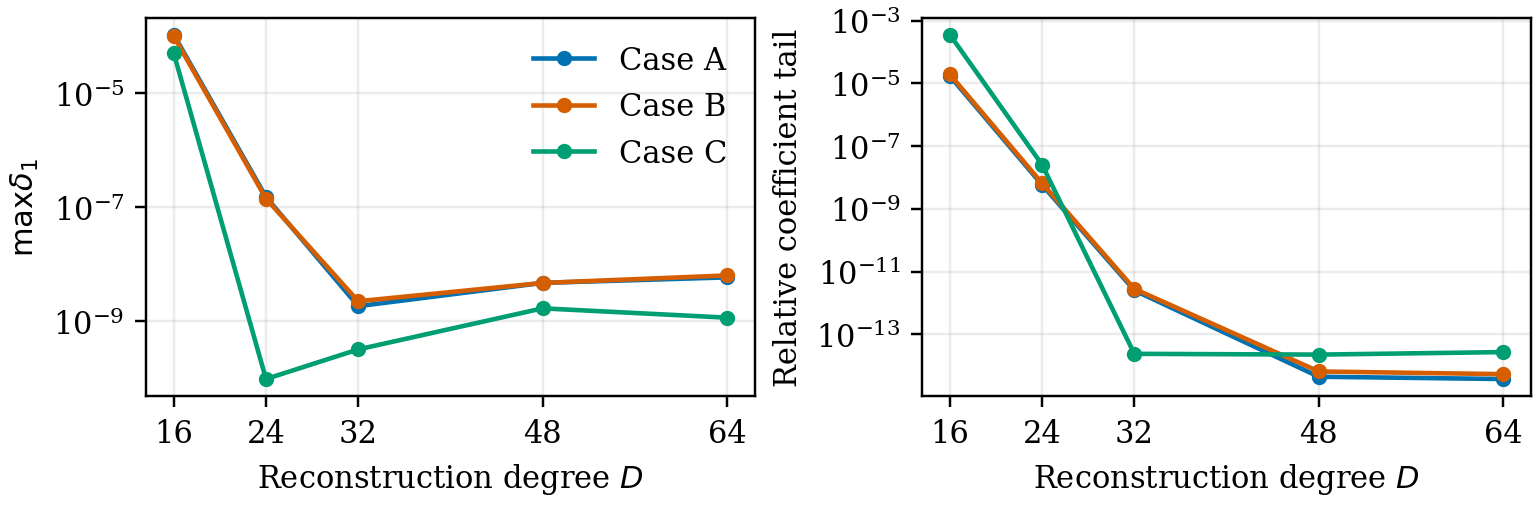
\includegraphics[width=0.95\textwidth]{../../figures/kerr_scalar_sourced_local_validation_20261008.png}
\caption{Independent local first-order-field validation.  Left: maximum
field-dependent sourced residual on $600$ validation nodes.  Right:
relative coefficient tail.  Cases and degrees are identical to
Table~\ref{tab:sourced20261008}.  The high-degree residual floor is shown
explicitly; a smaller coefficient tail does not guarantee a smaller
second-derivative residual.}
\label{fig:sourced20261008}
\end{figure*}
\subsection{Cancellation-free peeled coefficients}

Write $H=r^2+a^2$, $K=\omega H-am$, and
$p=\omega-m\Omega_H$.  If $R=Fu$, the coefficient multiplying $u$ is
\begin{equation}
B_0=\Delta(q'+q^2)+\Delta' q+K^2/\Delta-\lambda,
\qquad q=F'/F.
\end{equation}
For $F=r^{-1}\exp(i\sigma\omega r_*)$, $\sigma=\pm1$, direct substitution
and cancellation before floating-point evaluation give
\begin{equation}
\begin{split}
B_0^{\sigma}={}&\frac{am(am-2\omega H)}{\Delta}-\lambda
-\frac{2i\sigma\omega a^2}{r}\\
&-\frac{2M}{r}+\frac{2a^2}{r^2}.
\end{split}
\label{eq:outerfactored20261008}
\end{equation}
Consequently the exact infinity row is
$B_0(0)=-\lambda-2am\omega=-(A+a^2\omega^2)$, not $-\lambda$.
The difference vanishes for $m=0$ or $a=0$.
For $F=\exp(-ipr_*)$, the identity
$K-pH=(\omega-p)(r-r_+)(r+r_+)$ gives
\begin{equation}
B_0^{\mathrm{in}}=
\frac{(\omega-p)(r+r_+)(K+pH)}{r-r_-}
-2ipr-\lambda.
\label{eq:innerfactored20261008}
\end{equation}
This removes the apparent division by $r-r_+$ without moving the horizon
boundary.  The normalization remains $u(1)=1$ and the degenerate ODE row
remains in the matrix.  Neither expression changes the differential equation.

We tested $a/M=0.99,0.999$, $\ell=m=1,2$, and $n=1,2$ at
$p/\kappa=0.5$.  The spectral degrees were $128,176,224$, with
$r_{\rm match}/M=12$ and Gauss orders $2N$.  A further run at $N=224$
used the erroneous infinity row solely to quantify its effect.  The
corrected maximum homogeneous radial relative residual across these probes
was $3.2\times10^{-9}$; the maximum peeled-amplitude relative residual was
$5.2\times10^{-8}$.  Both denominators contain the corresponding field
terms.  The erroneous row changes the tested responses only at the
$10^{-8}$ level or below, but produces spurious outer spectral tails.
The freshly computed grid in Sec.~\ref{sec:principal20261014} uses
the corrected endpoint coefficients throughout.

At $a/M=0.999$, $\ell=m=2$, the $N=176\to224$ fractional change in the
cubic response was $1.6\times10^{-6}$ when the quadrature order also changed.
At fixed $N=224$, increasing the Gauss order from $448$ to $1792$ gives a
similar change, identifying quadrature as a separate error source.
Matching radii $8M,12M,16M$ were also checked independently.
These tests quantify consistency at the stated finite parameters.

\subsection{Local residual of the sourced field}

Let $Q=(r^2C_0+a^2C_2)|R_0|^{2n}R_0$ denote the projected source without
its minus sign, and $V=K^2/\Delta-\lambda$.  With unit-horizon $R_{\rm in}$
and unit-outgoing $R_{\rm up}$, reconstruct
\begin{equation}
R_1(r)=-\frac{R_{\rm up}(r)I_{\rm in}(r)
                    +R_{\rm in}(r)I_{\rm up}(r)}{W},
\end{equation}
where
\begin{align}
I_{\rm in}(r)&=\int_{r_+}^{r}R_{\rm in}(s)Q(s)\,ds,\\
I_{\rm up}(r)&=\int_r^\infty R_{\rm up}(s)Q(s)\,ds,\\
W&=\Delta(R_{\rm in}R_{\rm up}'-R_{\rm up}R_{\rm in}').
\end{align}
To avoid replacing a numerical test by a Green-function identity, we
evaluate these integrals at reconstruction nodes and differentiate their
Chebyshev interpolant, rather than setting $R_1''$ from the ODE.  The
independent local diagnostic is
\begin{equation}
\delta_1(r)=\frac{|\Delta R_1''+\Delta'R_1'+VR_1+Q|}
{|\Delta R_1''|+|\Delta'R_1'|+|VR_1|+|Q|}.
\label{eq:sourcedresidual20261008}
\end{equation}
The field factors in this denominator are essential for invariance under
a common rescaling of the first-order field and its source.

The homogeneous degree is $224$.  The initial horizon-to-$3M$ integrals
use $1024$ open Gauss nodes, the local cumulative increments use $128$
nodes, and the global outgoing-source integral retains the infinite-tail
calculation.  We reconstruct on $3M\le r\le8M$ with degrees
$16,24,32,48,64$ and validate at $600$ Chebyshev--Gauss points different
from the reconstruction nodes.  Cases A and B have $a/M=0.5$,
$\ell=m=0$, $M\omega=0.1$, with $n=1,2$, respectively.  Case C has
$a/M=0.99$, $\ell=m=2$, $p/\kappa=0.5$, and $n=1$.
Table~\ref{tab:sourced20261008} reports all reconstruction degrees;
none was selected by minimizing the residual after the calculation.

The decrease at low degree followed by a nonmonotonic floor is consistent
with spectral truncation giving way to numerical interpolation and
differentiation error.  At degree $32$, maxima are below
$2.3\times10^{-9}$ for all three cases.  This verifies the local sourced
equation on the stated interval, not the accuracy of the accumulated
homogeneous integration constants or the omitted asymptotic intervals.
Global flux/quadrature checks are still needed.  No global
machine-precision accuracy claim follows from this test.


\begin{thebibliography}{99}
\bibitem{Sanchez1976}
N.~G. Sanchez,
Scattering of scalar waves from a Schwarzschild black hole,
J. Math. Phys. \textbf{17}, 688 (1976).

\bibitem{Futterman}
J.~A. H. Futterman, F.~A. Handler, and R.~A. Matzner,
\textit{Scattering from Black Holes}
(Cambridge University Press, Cambridge, 1988).

\bibitem{GlampedakisAndersson2001}
K.~Glampedakis and N.~Andersson,
Scattering of scalar waves by rotating black holes,
Class. Quantum Grav. \textbf{18}, 1939 (2001).

\bibitem{Berti2009}
E.~Berti, V.~Cardoso, and A.~O. Starinets,
Quasinormal modes of black holes and black branes,
Class. Quantum Grav. \textbf{26}, 163001 (2009).

\bibitem{Kyutoku2023}
K.~Kyutoku, H.~Motohashi, and T.~Tanaka,
Quasinormal modes of Schwarzschild black holes on the real axis,
Phys. Rev. D \textbf{107}, 044012 (2023).

\bibitem{Rosato2024}
R.~F. Rosato, K.~Destounis, and P.~Pani,
Ringdown stability: Graybody factors as stable gravitational-wave observables,
Phys. Rev. D \textbf{110}, L121501 (2024).

\bibitem{Zlochower2003}
Y.~Zlochower, R.~G\'omez, S.~Husa, L.~Lehner, and J.~Winicour,
Mode coupling in the nonlinear response of black holes,
Phys. Rev. D \textbf{68}, 084014 (2003),
doi:10.1103/PhysRevD.68.084014,
arXiv:gr-qc/0306098.

\bibitem{Frauendiener2021}
J.~Frauendiener and C.~Stevens,
The non-linear perturbation of a black hole by gravitational waves. I. The
Bondi-Sachs mass loss,
Class. Quantum Grav. \textbf{38}, 194002 (2021).

\bibitem{YoshinoKodama2012}
H.~Yoshino and H.~Kodama,
Bosenova collapse of axion cloud around a rotating black hole,
Prog. Theor. Phys. \textbf{128}, 153 (2012),
doi:10.1143/PTP.128.153,
arXiv:1203.5070 [gr-qc].

\bibitem{Baryakhtar2021}
M.~Baryakhtar, M.~Galanis, R.~Lasenby, and O.~Simon,
Black hole superradiance of self-interacting scalar fields,
Phys. Rev. D \textbf{103}, 095019 (2021),
doi:10.1103/PhysRevD.103.095019,
arXiv:2011.11646 [hep-ph].

\bibitem{HerdeiroQCloud2014}
C.~Herdeiro, E.~Radu, and H.~R\'unarsson,
Non-linear $Q$-clouds around Kerr black holes,
Phys. Lett. B \textbf{739}, 302 (2014),
doi:10.1016/j.physletb.2014.11.005,
arXiv:1409.2877 [gr-qc].

\bibitem{BarackPound2019}
L.~Barack and A.~Pound,
Self-force and radiation reaction in general relativity,
Rep. Prog. Phys. \textbf{82}, 016904 (2019).

\bibitem{PoundWardell2021}
A.~Pound and B.~Wardell,
Black hole perturbation theory and gravitational self-force,
in \textit{Handbook of Gravitational Wave Astronomy}, edited by
C.~Bambi (Springer, Singapore, 2021), Chap.~38,
doi:10.1007/978-981-15-4702-7\_38-1,
arXiv:2101.04592 [gr-qc].

\bibitem{CardosoNonlinear2026}
V. Cardoso, J. Redondo-Yuste, U. Sperhake, and F. Tuncer,
Nonlinear Dynamics in General Relativity,
arXiv:2603.04501 [gr-qc] (2026).
\bibitem{GrallaTransient2016}
S. E. Gralla, A. Zimmerman, and P. Zimmerman,
Transient instability of rapidly rotating black holes,
Phys. Rev. D \textbf{94}, 084017 (2016),
doi:10.1103/PhysRevD.94.084017, arXiv:1608.04739 [gr-qc].
\bibitem{GrallaCritical2018}
S. E. Gralla and P. Zimmerman,
Critical exponents of extremal Kerr perturbations,
Class. Quantum Grav. \textbf{35}, 095002 (2018),
doi:10.1088/1361-6382/aab140, arXiv:1711.00855 [gr-qc].
\bibitem{IulianoWeather2025}
C. Iuliano, S. Hollands, S. R. Green, and P. Zimmerman,
Extremal black hole weather,
Phys. Rev. D \textbf{111}, 124038 (2025),
doi:10.1103/PhysRevD.111.124038, arXiv:2412.02821 [gr-qc].
\bibitem{HeTianZhangManuscript2026}
Z.-T. He, Y. Tian, and H. Zhang,
Nonlinear scattering problem in black hole spacetimes,
supplied manuscript, version dated June 15, 2026.
\bibitem{BredbergKerrCFT2010}
I.~Bredberg, T.~Hartman, W.~Song, and A.~Strominger,
Black hole superradiance from Kerr/CFT,
J. High Energy Phys. \textbf{04} (2010) 019,
doi:10.1007/JHEP04(2010)019,
arXiv:0907.3477 [hep-th].

\bibitem{Teukolsky1973}
S.~A. Teukolsky,
Perturbations of a rotating black hole. I. Fundamental equations for
gravitational, electromagnetic, and neutrino-field perturbations,
Astrophys. J. \textbf{185}, 635 (1973).

\bibitem{MST1996}
S.~Mano, H.~Suzuki, and E.~Takasugi,
Analytic solutions of the Teukolsky equation and their low frequency
expansions,
Prog. Theor. Phys. \textbf{95}, 1079 (1996),
arXiv:gr-qc/9603020.

\bibitem{ChungWagleYunes2023}
A.~K.-W. Chung, P.~Wagle, and N.~Yunes,
Spectral method for the gravitational perturbations of black holes:
Schwarzschild background case,
Phys. Rev. D \textbf{107}, 124032 (2023),
arXiv:2302.11624 [gr-qc].

\bibitem{Hughes2000}
S.~A. Hughes,
Computing radiation from Kerr black holes: Generalization of the
Sasaki--Nakamura equation,
Phys. Rev. D \textbf{61}, 084004 (2000),
arXiv:gr-qc/0002043.

\bibitem{Lo2023}
R.~K.~L. Lo,
Recipes for computing radiation from a Kerr black hole using a generalized
Sasaki--Nakamura formalism: Homogeneous solutions,
Phys. Rev. D \textbf{110}, 124070 (2024),
arXiv:2306.16469.

\bibitem{Hawking1975}
S.~W. Hawking,
Particle creation by black holes,
Commun. Math. Phys. \textbf{43}, 199 (1975).

\bibitem{Oshita2023}
N.~Oshita,
Thermal ringdown of a Kerr black hole: Overtone excitation, Fermi-Dirac
statistics and greybody factor,
JCAP \textbf{04}, 013 (2023).

\bibitem{Oshita2024}
N.~Oshita,
Greybody factors imprinted on black hole ringdowns: An alternative to
superposed quasinormal modes,
Phys. Rev. D \textbf{109}, 104028 (2024).

\bibitem{Stein2019}
L.~C. Stein,
qnm: A Python package for calculating Kerr quasinormal modes, separation
constants, and spherical-spheroidal mixing coefficients,
J. Open Source Softw. \textbf{4}, 1683 (2019).

\bibitem{GreenEtAl2023}
S.~R. Green, S.~Hollands, L.~Sberna, V.~Toomani, and P.~Zimmerman,
Conserved currents for a Kerr black hole and orthogonality of quasinormal
modes,
Phys. Rev. D \textbf{107}, 064030 (2023),
doi:10.1103/PhysRevD.107.064030,
arXiv:2210.15935 [gr-qc].

\end{thebibliography}
\end{document}
